% Options for packages loaded elsewhere
\PassOptionsToPackage{unicode}{hyperref}
\PassOptionsToPackage{hyphens}{url}
%
\documentclass[
]{article}
\usepackage{amsmath,amssymb}
\usepackage{iftex}
\ifPDFTeX
  \usepackage[T1]{fontenc}
  \usepackage[utf8]{inputenc}
  \usepackage{textcomp} % provide euro and other symbols
\else % if luatex or xetex
  \usepackage{unicode-math} % this also loads fontspec
  \defaultfontfeatures{Scale=MatchLowercase}
  \defaultfontfeatures[\rmfamily]{Ligatures=TeX,Scale=1}
\fi
\usepackage{lmodern}
\ifPDFTeX\else
  % xetex/luatex font selection
\fi
% Use upquote if available, for straight quotes in verbatim environments
\IfFileExists{upquote.sty}{\usepackage{upquote}}{}
\IfFileExists{microtype.sty}{% use microtype if available
  \usepackage[]{microtype}
  \UseMicrotypeSet[protrusion]{basicmath} % disable protrusion for tt fonts
}{}
\makeatletter
\@ifundefined{KOMAClassName}{% if non-KOMA class
  \IfFileExists{parskip.sty}{%
    \usepackage{parskip}
  }{% else
    \setlength{\parindent}{0pt}
    \setlength{\parskip}{6pt plus 2pt minus 1pt}}
}{% if KOMA class
  \KOMAoptions{parskip=half}}
\makeatother
\usepackage{xcolor}
\usepackage[margin=1in]{geometry}
\usepackage{color}
\usepackage{fancyvrb}
\newcommand{\VerbBar}{|}
\newcommand{\VERB}{\Verb[commandchars=\\\{\}]}
\DefineVerbatimEnvironment{Highlighting}{Verbatim}{commandchars=\\\{\}}
% Add ',fontsize=\small' for more characters per line
\usepackage{framed}
\definecolor{shadecolor}{RGB}{248,248,248}
\newenvironment{Shaded}{\begin{snugshade}}{\end{snugshade}}
\newcommand{\AlertTok}[1]{\textcolor[rgb]{0.94,0.16,0.16}{#1}}
\newcommand{\AnnotationTok}[1]{\textcolor[rgb]{0.56,0.35,0.01}{\textbf{\textit{#1}}}}
\newcommand{\AttributeTok}[1]{\textcolor[rgb]{0.13,0.29,0.53}{#1}}
\newcommand{\BaseNTok}[1]{\textcolor[rgb]{0.00,0.00,0.81}{#1}}
\newcommand{\BuiltInTok}[1]{#1}
\newcommand{\CharTok}[1]{\textcolor[rgb]{0.31,0.60,0.02}{#1}}
\newcommand{\CommentTok}[1]{\textcolor[rgb]{0.56,0.35,0.01}{\textit{#1}}}
\newcommand{\CommentVarTok}[1]{\textcolor[rgb]{0.56,0.35,0.01}{\textbf{\textit{#1}}}}
\newcommand{\ConstantTok}[1]{\textcolor[rgb]{0.56,0.35,0.01}{#1}}
\newcommand{\ControlFlowTok}[1]{\textcolor[rgb]{0.13,0.29,0.53}{\textbf{#1}}}
\newcommand{\DataTypeTok}[1]{\textcolor[rgb]{0.13,0.29,0.53}{#1}}
\newcommand{\DecValTok}[1]{\textcolor[rgb]{0.00,0.00,0.81}{#1}}
\newcommand{\DocumentationTok}[1]{\textcolor[rgb]{0.56,0.35,0.01}{\textbf{\textit{#1}}}}
\newcommand{\ErrorTok}[1]{\textcolor[rgb]{0.64,0.00,0.00}{\textbf{#1}}}
\newcommand{\ExtensionTok}[1]{#1}
\newcommand{\FloatTok}[1]{\textcolor[rgb]{0.00,0.00,0.81}{#1}}
\newcommand{\FunctionTok}[1]{\textcolor[rgb]{0.13,0.29,0.53}{\textbf{#1}}}
\newcommand{\ImportTok}[1]{#1}
\newcommand{\InformationTok}[1]{\textcolor[rgb]{0.56,0.35,0.01}{\textbf{\textit{#1}}}}
\newcommand{\KeywordTok}[1]{\textcolor[rgb]{0.13,0.29,0.53}{\textbf{#1}}}
\newcommand{\NormalTok}[1]{#1}
\newcommand{\OperatorTok}[1]{\textcolor[rgb]{0.81,0.36,0.00}{\textbf{#1}}}
\newcommand{\OtherTok}[1]{\textcolor[rgb]{0.56,0.35,0.01}{#1}}
\newcommand{\PreprocessorTok}[1]{\textcolor[rgb]{0.56,0.35,0.01}{\textit{#1}}}
\newcommand{\RegionMarkerTok}[1]{#1}
\newcommand{\SpecialCharTok}[1]{\textcolor[rgb]{0.81,0.36,0.00}{\textbf{#1}}}
\newcommand{\SpecialStringTok}[1]{\textcolor[rgb]{0.31,0.60,0.02}{#1}}
\newcommand{\StringTok}[1]{\textcolor[rgb]{0.31,0.60,0.02}{#1}}
\newcommand{\VariableTok}[1]{\textcolor[rgb]{0.00,0.00,0.00}{#1}}
\newcommand{\VerbatimStringTok}[1]{\textcolor[rgb]{0.31,0.60,0.02}{#1}}
\newcommand{\WarningTok}[1]{\textcolor[rgb]{0.56,0.35,0.01}{\textbf{\textit{#1}}}}
\usepackage{graphicx}
\makeatletter
\def\maxwidth{\ifdim\Gin@nat@width>\linewidth\linewidth\else\Gin@nat@width\fi}
\def\maxheight{\ifdim\Gin@nat@height>\textheight\textheight\else\Gin@nat@height\fi}
\makeatother
% Scale images if necessary, so that they will not overflow the page
% margins by default, and it is still possible to overwrite the defaults
% using explicit options in \includegraphics[width, height, ...]{}
\setkeys{Gin}{width=\maxwidth,height=\maxheight,keepaspectratio}
% Set default figure placement to htbp
\makeatletter
\def\fps@figure{htbp}
\makeatother
\usepackage{soul}
\setlength{\emergencystretch}{3em} % prevent overfull lines
\providecommand{\tightlist}{%
  \setlength{\itemsep}{0pt}\setlength{\parskip}{0pt}}
\setcounter{secnumdepth}{-\maxdimen} % remove section numbering
\usepackage{booktabs}
\usepackage{longtable}
\usepackage{array}
\usepackage{multirow}
\usepackage{wrapfig}
\usepackage{float}
\usepackage{colortbl}
\usepackage{pdflscape}
\usepackage{tabu}
\usepackage{threeparttable}
\usepackage{threeparttablex}
\usepackage[normalem]{ulem}
\usepackage{makecell}
\usepackage{xcolor}
\ifLuaTeX
  \usepackage{selnolig}  % disable illegal ligatures
\fi
\IfFileExists{bookmark.sty}{\usepackage{bookmark}}{\usepackage{hyperref}}
\IfFileExists{xurl.sty}{\usepackage{xurl}}{} % add URL line breaks if available
\urlstyle{same}
\hypersetup{
  pdftitle={Submission},
  hidelinks,
  pdfcreator={LaTeX via pandoc}}

\title{Submission}
\author{}
\date{\vspace{-2.5em}}

\begin{document}
\maketitle

{
\setcounter{tocdepth}{2}
\tableofcontents
}
\hypertarget{background}{%
\section{Background}\label{background}}

\hypertarget{what-is-biliary-cholangitis}{%
\subsection{What is Biliary
Cholangitis?}\label{what-is-biliary-cholangitis}}

Primary Biliary Cholangitis (previously called Primary Biliary
Cirrhosis) is an autoimmune disease where bile ducts become swollen and
inflamed and block the flow of bile. Bile is a substance that aids with
digestion. The bile ducts carry bile from the liver to the small
intestine. The swelling and inflammation can lead to scarring of the
liver which is cirrhosis. Advanced cirrhosis can lead to liver failure
or liver cancer. Medication can slow progression. There is no definite
cure at this time.

\begin{figure}
\centering
\includegraphics{17715-primary-biliary-cholangitis.webp}
\caption{\ul{Primary Biliary Cholangitis
(\href{https://www.google.com/search?client=safari\&sca_esv=591276386\&rls=en\&sxsrf=AM9HkKmtJVOC2Jrf2BSYVB2O-QcnTSgx6g:1702664705100\&q=Primary+Biliary+Cholangitis\&tbm=isch\&source=lnms\&sa=X\&ved=2ahUKEwid0qyniJKDAxX9FFkFHVH3CcoQ0pQJegQIDxAB\&biw=1440\&bih=848\&dpr=2\#imgrc=UeV_fhP-8vPOlM}{Source})}}
\end{figure}

\hypertarget{objectives}{%
\subsection{Objectives}\label{objectives}}

\hypertarget{q1-what-predictors-if-any-increases-an-individuals-chance-of-receiving-a-liver-transplant}{%
\subsubsection{Q1: What predictors, if any, increases an individual's
chance of receiving a liver
transplant?}\label{q1-what-predictors-if-any-increases-an-individuals-chance-of-receiving-a-liver-transplant}}

\hypertarget{q2-are-there-factors-not-currently-included-in-medical-definition-that-can-help-distinguish-different-stages-of-biliary-cholangitis}{%
\subsubsection{Q2: Are there factors not currently included in medical
definition that can help distinguish different stages of Biliary
Cholangitis?}\label{q2-are-there-factors-not-currently-included-in-medical-definition-that-can-help-distinguish-different-stages-of-biliary-cholangitis}}

\hypertarget{clinical-study-dataset-background}{%
\subsection{Clinical Study + Dataset Background
:}\label{clinical-study-dataset-background}}

The dataset is produced from a clinical study by Mayo Clinic run from
1974-1984. The final `Status' of each patient was observed in 1986.
`Status' was either Dead, Censored, or Censored due to liver transplant.

A link to the original study is here:
\url{https://faculty.washington.edu/abansal/ShortCourse_DynamicDecisionMaking/Dickson1989_MayoPBCOriginalArticle.pdf}

\hypertarget{load-in-packages}{%
\subsubsection{Load in Packages}\label{load-in-packages}}

\begin{Shaded}
\begin{Highlighting}[]
\FunctionTok{library}\NormalTok{(survival)}
\FunctionTok{library}\NormalTok{(ggplot2)}
\FunctionTok{library}\NormalTok{(survival)}
\FunctionTok{library}\NormalTok{(survminer)}
\end{Highlighting}
\end{Shaded}

\begin{verbatim}
## Loading required package: ggpubr
\end{verbatim}

\begin{verbatim}
## 
## Attaching package: 'survminer'
\end{verbatim}

\begin{verbatim}
## The following object is masked from 'package:survival':
## 
##     myeloma
\end{verbatim}

\begin{Shaded}
\begin{Highlighting}[]
\FunctionTok{library}\NormalTok{(kableExtra)}
\FunctionTok{library}\NormalTok{(factoextra)}
\end{Highlighting}
\end{Shaded}

\begin{verbatim}
## Welcome! Want to learn more? See two factoextra-related books at https://goo.gl/ve3WBa
\end{verbatim}

\hypertarget{data-processing}{%
\subsubsection{Data Processing}\label{data-processing}}

\begin{Shaded}
\begin{Highlighting}[]
\CommentTok{\#load in the data}
\FunctionTok{library}\NormalTok{(tidyverse)}
\end{Highlighting}
\end{Shaded}

\begin{verbatim}
## -- Attaching core tidyverse packages ------------------------ tidyverse 2.0.0 --
## v dplyr     1.1.3     v readr     2.1.4
## v forcats   1.0.0     v stringr   1.5.0
## v lubridate 1.9.2     v tibble    3.2.1
## v purrr     1.0.2     v tidyr     1.3.0
## -- Conflicts ------------------------------------------ tidyverse_conflicts() --
## x dplyr::filter()     masks stats::filter()
## x dplyr::group_rows() masks kableExtra::group_rows()
## x dplyr::lag()        masks stats::lag()
## i Use the conflicted package (<http://conflicted.r-lib.org/>) to force all conflicts to become errors
\end{verbatim}

\begin{Shaded}
\begin{Highlighting}[]
\CommentTok{\#load data}
\NormalTok{cirrhosis }\OtherTok{\textless{}{-}} \FunctionTok{read\_csv}\NormalTok{(}\StringTok{"cirrhosis.csv"}\NormalTok{)}
\end{Highlighting}
\end{Shaded}

\begin{verbatim}
## Rows: 418 Columns: 20
## -- Column specification --------------------------------------------------------
## Delimiter: ","
## chr  (7): Status, Drug, Sex, Ascites, Hepatomegaly, Spiders, Edema
## dbl (13): ID, N_Days, Age, Bilirubin, Cholesterol, Albumin, Copper, Alk_Phos...
## 
## i Use `spec()` to retrieve the full column specification for this data.
## i Specify the column types or set `show_col_types = FALSE` to quiet this message.
\end{verbatim}

\begin{Shaded}
\begin{Highlighting}[]
\FunctionTok{head}\NormalTok{(cirrhosis)}
\end{Highlighting}
\end{Shaded}

\begin{verbatim}
## # A tibble: 6 x 20
##      ID N_Days Status Drug          Age Sex   Ascites Hepatomegaly Spiders Edema
##   <dbl>  <dbl> <chr>  <chr>       <dbl> <chr> <chr>   <chr>        <chr>   <chr>
## 1     1    400 D      D-penicill~ 21464 F     Y       Y            Y       Y    
## 2     2   4500 C      D-penicill~ 20617 F     N       Y            Y       N    
## 3     3   1012 D      D-penicill~ 25594 M     N       N            N       S    
## 4     4   1925 D      D-penicill~ 19994 F     N       Y            Y       S    
## 5     5   1504 CL     Placebo     13918 F     N       Y            Y       N    
## 6     6   2503 D      Placebo     24201 F     N       Y            N       N    
## # i 10 more variables: Bilirubin <dbl>, Cholesterol <dbl>, Albumin <dbl>,
## #   Copper <dbl>, Alk_Phos <dbl>, SGOT <dbl>, Tryglicerides <dbl>,
## #   Platelets <dbl>, Prothrombin <dbl>, Stage <dbl>
\end{verbatim}

\hypertarget{pre-process-the-data}{%
\subsubsection{Pre-process the data}\label{pre-process-the-data}}

\begin{Shaded}
\begin{Highlighting}[]
\CommentTok{\#encode the sex, ascites, hepatomegaly, spiders, edema into binary variables}
\NormalTok{cirrhosis}\SpecialCharTok{$}\NormalTok{Sex }\OtherTok{\textless{}{-}} \FunctionTok{ifelse}\NormalTok{(cirrhosis}\SpecialCharTok{$}\NormalTok{Sex }\SpecialCharTok{==} \StringTok{"F"}\NormalTok{, }\DecValTok{0}\NormalTok{, }\DecValTok{1}\NormalTok{)}
\NormalTok{cirrhosis}\SpecialCharTok{$}\NormalTok{Ascites }\OtherTok{\textless{}{-}} \FunctionTok{ifelse}\NormalTok{(cirrhosis}\SpecialCharTok{$}\NormalTok{Ascites }\SpecialCharTok{==} \StringTok{"Y"}\NormalTok{, }\DecValTok{1}\NormalTok{, }\DecValTok{0}\NormalTok{)}
\NormalTok{cirrhosis}\SpecialCharTok{$}\NormalTok{Hepatomegaly }\OtherTok{\textless{}{-}} \FunctionTok{ifelse}\NormalTok{(cirrhosis}\SpecialCharTok{$}\NormalTok{Hepatomegaly }\SpecialCharTok{==} \StringTok{"Y"}\NormalTok{, }\DecValTok{1}\NormalTok{, }\DecValTok{0}\NormalTok{)}
\NormalTok{cirrhosis}\SpecialCharTok{$}\NormalTok{Spiders }\OtherTok{\textless{}{-}} \FunctionTok{ifelse}\NormalTok{(cirrhosis}\SpecialCharTok{$}\NormalTok{Spiders }\SpecialCharTok{==} \StringTok{"Y"}\NormalTok{, }\DecValTok{1}\NormalTok{, }\DecValTok{0}\NormalTok{)}
\CommentTok{\#factorize the stage}
\NormalTok{cirrhosis}\SpecialCharTok{$}\NormalTok{Stage }\OtherTok{\textless{}{-}} \FunctionTok{factor}\NormalTok{(cirrhosis}\SpecialCharTok{$}\NormalTok{Stage)}
\NormalTok{cirrhosis}\SpecialCharTok{$}\NormalTok{Status }\OtherTok{\textless{}{-}} \FunctionTok{factor}\NormalTok{(cirrhosis}\SpecialCharTok{$}\NormalTok{Status)}
\NormalTok{cirrhosis}\SpecialCharTok{$}\NormalTok{Drug }\OtherTok{\textless{}{-}} \FunctionTok{factor}\NormalTok{(cirrhosis}\SpecialCharTok{$}\NormalTok{Drug)}
\NormalTok{cirrhosis}\SpecialCharTok{$}\NormalTok{Sex }\OtherTok{\textless{}{-}} \FunctionTok{factor}\NormalTok{(cirrhosis}\SpecialCharTok{$}\NormalTok{Sex)}
\CommentTok{\#cirrhosis$Ascites \textless{}{-} factor(cirrhosis$Ascites)}
\CommentTok{\#cirrhosis$Hepatomegaly \textless{}{-} factor(cirrhosis$Hepatomegaly)}
\CommentTok{\#cirrhosis$Spiders \textless{}{-} factor(cirrhosis$Spiders)}
\NormalTok{cirrhosis}\SpecialCharTok{$}\NormalTok{Edema }\OtherTok{\textless{}{-}} \FunctionTok{factor}\NormalTok{(cirrhosis}\SpecialCharTok{$}\NormalTok{Edema)}
\NormalTok{cirrhosis}\SpecialCharTok{$}\NormalTok{Sex }\OtherTok{\textless{}{-}} \FunctionTok{factor}\NormalTok{(}\FunctionTok{ifelse}\NormalTok{(cirrhosis}\SpecialCharTok{$}\NormalTok{Sex }\SpecialCharTok{==} \DecValTok{0}\NormalTok{, }\StringTok{"Female"}\NormalTok{, }\StringTok{"Male"}\NormalTok{))}

\CommentTok{\#Drop the first column}
\NormalTok{cirrhosis }\OtherTok{\textless{}{-}}\NormalTok{ cirrhosis[,}\SpecialCharTok{{-}}\DecValTok{1}\NormalTok{]}
\end{Highlighting}
\end{Shaded}

\begin{itemize}
\item
  Engage in Exploratory Data Analysis
\item
  Use Machine Learning Algorithms:

  \begin{itemize}
  \tightlist
  \item
    You must use at least one of each: a Regression-based algorithm, a
    Tree-based algorithm, and an Unsupervised Learning algorithm.
  \item
    Each algorithm must be explained for a general audience.
  \item
    All results should be explained.
  \item
    Where appropriate, comparisons between methods should be discussed.
    This includes highlighting the strengths and weaknesses of the
    various approaches as well as when each is appropriate.
  \end{itemize}
\item
  A discussion of what you've learned from your work about the context
  and recommendations for future work.
\item
  Author Contributions--list out who did what in the project.
\item
  References--Citation style is your choice, but all sources should be
  documented (both in text and in the References section). This includes
  where you got your data.
\item
  A commented Code Appendix
\end{itemize}

\begin{Shaded}
\begin{Highlighting}[]
\NormalTok{cirrhosis }\SpecialCharTok{\%\textgreater{}\%} 
  \FunctionTok{ggplot}\NormalTok{(}\FunctionTok{aes}\NormalTok{(}\AttributeTok{x =}\NormalTok{ N\_Days)) }\SpecialCharTok{+} \FunctionTok{geom\_histogram}\NormalTok{() }\SpecialCharTok{+}
  \FunctionTok{facet\_wrap}\NormalTok{(}\AttributeTok{facets =} \FunctionTok{vars}\NormalTok{(Status))}
\end{Highlighting}
\end{Shaded}

\begin{verbatim}
## `stat_bin()` using `bins = 30`. Pick better value with `binwidth`.
\end{verbatim}

\includegraphics{Submission_files/figure-latex/unnamed-chunk-9-1.pdf}

\begin{Shaded}
\begin{Highlighting}[]
\CommentTok{\#Required libraries}
\FunctionTok{library}\NormalTok{(survival)}
\FunctionTok{library}\NormalTok{(ggplot2)}
\FunctionTok{library}\NormalTok{(survival)}
\FunctionTok{library}\NormalTok{(survminer)}
\end{Highlighting}
\end{Shaded}

\hypertarget{eda}{%
\section{EDA}\label{eda}}

\hypertarget{exploring-the-demographics-of-the-patients}{%
\subsection{Exploring the demographics of the
patients}\label{exploring-the-demographics-of-the-patients}}

\hypertarget{sex-ratio-of-patients}{%
\subsubsection{Sex Ratio of Patients}\label{sex-ratio-of-patients}}

\begin{Shaded}
\begin{Highlighting}[]
\CommentTok{\#cirrhosis$Sex \textless{}{-} factor(ifelse(cirrhosis$Sex == 0, "Female", "Male"))}

\CommentTok{\# Preparing the data for pie chart}
\NormalTok{sex\_data }\OtherTok{\textless{}{-}}\NormalTok{ cirrhosis }\SpecialCharTok{\%\textgreater{}\%} 
            \FunctionTok{count}\NormalTok{(Sex) }\SpecialCharTok{\%\textgreater{}\%} 
            \FunctionTok{mutate}\NormalTok{(}\AttributeTok{Percentage =}\NormalTok{ n }\SpecialCharTok{/} \FunctionTok{sum}\NormalTok{(n) }\SpecialCharTok{*} \DecValTok{100}\NormalTok{)}

\CommentTok{\# Pie Chart}
\FunctionTok{ggplot}\NormalTok{(sex\_data, }\FunctionTok{aes}\NormalTok{(}\AttributeTok{x=}\StringTok{""}\NormalTok{, }\AttributeTok{y=}\NormalTok{Percentage, }\AttributeTok{fill=}\NormalTok{Sex)) }\SpecialCharTok{+}
    \FunctionTok{geom\_bar}\NormalTok{(}\AttributeTok{stat=}\StringTok{"identity"}\NormalTok{, }\AttributeTok{width=}\DecValTok{1}\NormalTok{) }\SpecialCharTok{+}
    \FunctionTok{coord\_polar}\NormalTok{(}\StringTok{"y"}\NormalTok{, }\AttributeTok{start=}\DecValTok{0}\NormalTok{) }\SpecialCharTok{+}
    \FunctionTok{scale\_fill\_brewer}\NormalTok{(}\AttributeTok{palette=}\StringTok{"Pastel1"}\NormalTok{) }\SpecialCharTok{+}
    \FunctionTok{theme\_minimal}\NormalTok{() }\SpecialCharTok{+}
    \FunctionTok{theme}\NormalTok{(}\AttributeTok{axis.line =} \FunctionTok{element\_blank}\NormalTok{(),}
          \AttributeTok{axis.text =} \FunctionTok{element\_blank}\NormalTok{(),}
          \AttributeTok{axis.ticks =} \FunctionTok{element\_blank}\NormalTok{(),}
          \AttributeTok{panel.grid =} \FunctionTok{element\_blank}\NormalTok{(),}
          \AttributeTok{plot.title =} \FunctionTok{element\_text}\NormalTok{(}\AttributeTok{size=}\DecValTok{14}\NormalTok{, }\AttributeTok{face=}\StringTok{"bold"}\NormalTok{)) }\SpecialCharTok{+}
    \FunctionTok{labs}\NormalTok{(}\AttributeTok{fill=}\StringTok{"Sex"}\NormalTok{, }\AttributeTok{title=}\StringTok{" Sex Amongst Patients"}\NormalTok{)}
\end{Highlighting}
\end{Shaded}

\includegraphics{Submission_files/figure-latex/unnamed-chunk-11-1.pdf}

Primary Biliary Cholangitis affects women much more than men at a 10-1
ratio. The data of this clinical study mimics the greater population.
Investigating gender-based differences in disease progression can
uncover any gender-specific patterns in PBC. This could lead to
gender-tailored treatment approaches and a better understanding of the
disease's biology, which might differ between males and females.

\hypertarget{age-distribution-of-patients}{%
\subsubsection{Age Distribution of
Patients}\label{age-distribution-of-patients}}

\begin{Shaded}
\begin{Highlighting}[]
\CommentTok{\# Converting age from days to years for better readability}
\NormalTok{cirrhosis}\SpecialCharTok{$}\NormalTok{Age\_Years }\OtherTok{\textless{}{-}}\NormalTok{ cirrhosis}\SpecialCharTok{$}\NormalTok{Age }\SpecialCharTok{/} \FloatTok{365.25}

\CommentTok{\# Histogram}
\FunctionTok{ggplot}\NormalTok{(cirrhosis, }\FunctionTok{aes}\NormalTok{(}\AttributeTok{x=}\NormalTok{Age\_Years)) }\SpecialCharTok{+}
    \FunctionTok{geom\_histogram}\NormalTok{(}\AttributeTok{binwidth=}\DecValTok{5}\NormalTok{, }\AttributeTok{fill=}\StringTok{"\#69b3a2"}\NormalTok{, }\AttributeTok{color=}\StringTok{"\#e9ecef"}\NormalTok{) }\SpecialCharTok{+}
    \FunctionTok{theme\_minimal}\NormalTok{() }\SpecialCharTok{+}
    \FunctionTok{labs}\NormalTok{(}\AttributeTok{title=}\StringTok{"Age Distribution of PBC Patients"}\NormalTok{, }\AttributeTok{x=}\StringTok{"Age (years)"}\NormalTok{, }\AttributeTok{y=}\StringTok{"Count"}\NormalTok{) }\SpecialCharTok{+}
    \FunctionTok{theme}\NormalTok{(}\AttributeTok{plot.title =} \FunctionTok{element\_text}\NormalTok{(}\AttributeTok{size=}\DecValTok{14}\NormalTok{, }\AttributeTok{face=}\StringTok{"bold"}\NormalTok{))}
\end{Highlighting}
\end{Shaded}

\includegraphics{Submission_files/figure-latex/unnamed-chunk-12-1.pdf}

The distribution of ages is quite normal.

\hypertarget{looking-at-the-data-itself}{%
\subsection{Looking at the data
itself}\label{looking-at-the-data-itself}}

\hypertarget{na-counts-amongst-our-variables}{%
\subsubsection{NA counts amongst our
variables}\label{na-counts-amongst-our-variables}}

\begin{Shaded}
\begin{Highlighting}[]
\NormalTok{count }\OtherTok{\textless{}{-}}  \FunctionTok{data.frame}\NormalTok{(}\AttributeTok{NA\_CountsPerVar =} \FunctionTok{colSums}\NormalTok{(}\FunctionTok{is.na}\NormalTok{(cirrhosis)))}
\FunctionTok{kable}\NormalTok{(count)}
\end{Highlighting}
\end{Shaded}

\begin{tabular}{l|r}
\hline
  & NA\_CountsPerVar\\
\hline
N\_Days & 0\\
\hline
Status & 0\\
\hline
Drug & 106\\
\hline
Age & 0\\
\hline
Sex & 0\\
\hline
Ascites & 106\\
\hline
Hepatomegaly & 106\\
\hline
Spiders & 106\\
\hline
Edema & 0\\
\hline
Bilirubin & 0\\
\hline
Cholesterol & 134\\
\hline
Albumin & 0\\
\hline
Copper & 108\\
\hline
Alk\_Phos & 106\\
\hline
SGOT & 106\\
\hline
Tryglicerides & 136\\
\hline
Platelets & 11\\
\hline
Prothrombin & 2\\
\hline
Stage & 6\\
\hline
Age\_Years & 0\\
\hline
\end{tabular}

An observation is that many of the variables have 106 NAs. This
indicates that a good fraction {[}106 patients{]} were equally tracked
and measured in a less extensive way.

\hypertarget{distribution-of-stages-of-biliary-cholangitis}{%
\subsection{Distribution of Stages of Biliary
Cholangitis}\label{distribution-of-stages-of-biliary-cholangitis}}

\begin{Shaded}
\begin{Highlighting}[]
\NormalTok{cirrhosis }\SpecialCharTok{\%\textgreater{}\%}
      \FunctionTok{ggplot}\NormalTok{(}\FunctionTok{aes}\NormalTok{(}\AttributeTok{x =}\NormalTok{ Stage)) }\SpecialCharTok{+} \FunctionTok{geom\_bar}\NormalTok{(}\AttributeTok{fill =} \StringTok{"\#097969"}\NormalTok{) }\CommentTok{\# need color}
\end{Highlighting}
\end{Shaded}

\includegraphics{Submission_files/figure-latex/unnamed-chunk-14-1.pdf}

This distribution is left skewed and not symmetric. Most patients have
stage 3 and then 4 of Biliary Cholangitis.

\hypertarget{exploring-some-interactions-of-variables}{%
\subsection{Exploring some interactions of
variables}\label{exploring-some-interactions-of-variables}}

\hypertarget{how-does-prescense-of-a-d-penicillamine-with-stage-of-biliary-cholangitis-impact-number-of-days-till-death}{%
\subsubsection{How does prescense of a D-penicillamine with stage of
Biliary Cholangitis impact number of days till
death?}\label{how-does-prescense-of-a-d-penicillamine-with-stage-of-biliary-cholangitis-impact-number-of-days-till-death}}

\begin{Shaded}
\begin{Highlighting}[]
\FunctionTok{ggplot}\NormalTok{(}\AttributeTok{data =}\NormalTok{ cirrhosis, }\FunctionTok{aes}\NormalTok{ (Drug, Stage, }\AttributeTok{fill =}\NormalTok{ N\_Days))}\SpecialCharTok{+} \FunctionTok{geom\_tile}\NormalTok{() }\SpecialCharTok{+} \FunctionTok{scale\_fill\_distiller}\NormalTok{(}\AttributeTok{palette =} \StringTok{"RdPu"}\NormalTok{, }\AttributeTok{trans =} \StringTok{"reverse"}\NormalTok{) }
\end{Highlighting}
\end{Shaded}

\includegraphics{Submission_files/figure-latex/unnamed-chunk-15-1.pdf}

This heat map shows that being a placebo in stage 1 gives you a greater
amount of days till death in this sample of patients.

\hypertarget{individuals-with-edema-and-if-they-were-on-the-drug}{%
\subsubsection{Individuals with Edema, and if they were on the
drug}\label{individuals-with-edema-and-if-they-were-on-the-drug}}

\begin{Shaded}
\begin{Highlighting}[]
\NormalTok{hi }\OtherTok{=} \FunctionTok{c}\NormalTok{(}\StringTok{"\#40B5AD"}\NormalTok{, }\StringTok{"\#009E60"}\NormalTok{, }\StringTok{"\#9FE2BF"}\NormalTok{)}
\FunctionTok{library}\NormalTok{(ggmosaic)}
\NormalTok{cirrhosis }\SpecialCharTok{\%\textgreater{}\%}
  \FunctionTok{ggplot}\NormalTok{() }\SpecialCharTok{+}
  \FunctionTok{geom\_mosaic}\NormalTok{(}\FunctionTok{aes}\NormalTok{( }\AttributeTok{x =} \FunctionTok{product}\NormalTok{(Edema), }\AttributeTok{fill =}\NormalTok{ Drug)) }\SpecialCharTok{+} \FunctionTok{scale\_fill\_manual}\NormalTok{(}\AttributeTok{values =}\NormalTok{ hi)}
\end{Highlighting}
\end{Shaded}

\begin{verbatim}
## Warning: `unite_()` was deprecated in tidyr 1.2.0.
## i Please use `unite()` instead.
## i The deprecated feature was likely used in the ggmosaic package.
##   Please report the issue at <https://github.com/haleyjeppson/ggmosaic>.
## This warning is displayed once every 8 hours.
## Call `lifecycle::last_lifecycle_warnings()` to see where this warning was
## generated.
\end{verbatim}

\includegraphics{Submission_files/figure-latex/unnamed-chunk-16-1.pdf}

Edema is swelling due to too much liquid trapped in the body's tissues.
It's common complication in liver diseases and can significantly impact
patient quality of life and survival. Understanding how different levels
of edema (none, controlled by diuretics, or persistent despite
treatment) affect survival can inform patient management strategies and
highlight the need for aggressive interventions in certain cases. From
the graph we can see a even split between the placebo and drug for Edema
status. There is no NA values for Edema persistent despite diuretics. We
cannot directly compare it the splits for other statuses given their NA
values if known could change the look of the graph.

\hypertarget{mihir-choose-your-preffered-graph-and-explain}{%
\subsubsection{mihir choose your preffered graph and
explain}\label{mihir-choose-your-preffered-graph-and-explain}}

\hypertarget{survival-analysis-based-on-treatment-and-stage-how-does-the-survival-rate-differ-among-patients-at-different-stages-of-pbc-who-received-d-penicillamine-versus-placebo}{%
\subsubsection{Survival Analysis Based on Treatment and Stage: How does
the survival rate differ among patients at different stages of PBC who
received D-penicillamine versus
placebo?}\label{survival-analysis-based-on-treatment-and-stage-how-does-the-survival-rate-differ-among-patients-at-different-stages-of-pbc-who-received-d-penicillamine-versus-placebo}}

This question investigates the effectiveness of the drug D-penicillamine
compared to a placebo, considering the stage of PBC. By analyzing
survival rates across different disease stages and treatment types, we
can assess the drug's effectiveness at various disease stages. This
information is vital for clinicians to make informed decisions about
treatment plans and for researchers to understand the drug's impact.
(LOLL this is what the study acc sought to discover)

\begin{Shaded}
\begin{Highlighting}[]
\NormalTok{surv\_object }\OtherTok{\textless{}{-}} \FunctionTok{Surv}\NormalTok{(cirrhosis}\SpecialCharTok{$}\NormalTok{N\_Days, cirrhosis}\SpecialCharTok{$}\NormalTok{Status }\SpecialCharTok{==} \StringTok{\textquotesingle{}D\textquotesingle{}}\NormalTok{)}
\NormalTok{surv\_fit }\OtherTok{\textless{}{-}} \FunctionTok{survfit}\NormalTok{(surv\_object }\SpecialCharTok{\textasciitilde{}}\NormalTok{ cirrhosis}\SpecialCharTok{$}\NormalTok{Drug }\SpecialCharTok{+}\NormalTok{ cirrhosis}\SpecialCharTok{$}\NormalTok{Stage, }\AttributeTok{data =}\NormalTok{ cirrhosis)}
\FunctionTok{ggsurvplot}\NormalTok{(surv\_fit, }
           \AttributeTok{data =}\NormalTok{ cirrhosis,}
           \AttributeTok{conf.int =} \ConstantTok{TRUE}\NormalTok{, }
           \CommentTok{\#palette = c("\#00AFBB", "\#E7B800", "\#FC4E07"),}
           \AttributeTok{xlab =} \StringTok{"Days"}\NormalTok{, }
           \AttributeTok{ylab =} \StringTok{"Survival Probability"}\NormalTok{, }
           \AttributeTok{title =} \StringTok{"Survival Curves by Treatment and Stage"}\NormalTok{)}
\end{Highlighting}
\end{Shaded}

\includegraphics{Submission_files/figure-latex/unnamed-chunk-17-1.pdf}

\hypertarget{impact-of-liver-complications-on-survival-how-do-the-presence-of-ascites-hepatomegaly-and-spiders-relate-to-survival-time}{%
\subsubsection{Impact of Liver Complications on Survival: How do the
presence of ascites, hepatomegaly, and spiders relate to survival
time?}\label{impact-of-liver-complications-on-survival-how-do-the-presence-of-ascites-hepatomegaly-and-spiders-relate-to-survival-time}}

Exploring how liver-related symptoms (ascites, hepatomegaly, and
spiders) affect patient survival provides insights into the severity of
these complications in PBC progression. This can help in identifying
high-risk patients and understanding the disease's impact on liver
function.

\begin{Shaded}
\begin{Highlighting}[]
\NormalTok{surv\_fit\_complications }\OtherTok{\textless{}{-}} \FunctionTok{survfit}\NormalTok{(surv\_object }\SpecialCharTok{\textasciitilde{}}\NormalTok{ cirrhosis}\SpecialCharTok{$}\NormalTok{Ascites }\SpecialCharTok{+}\NormalTok{ cirrhosis}\SpecialCharTok{$}\NormalTok{Hepatomegaly }\SpecialCharTok{+}\NormalTok{ cirrhosis}\SpecialCharTok{$}\NormalTok{Spiders, }\AttributeTok{data =}\NormalTok{ cirrhosis)}
\FunctionTok{ggsurvplot}\NormalTok{(surv\_fit\_complications, }
           \AttributeTok{data =}\NormalTok{ cirrhosis,}
           \AttributeTok{conf.int =} \ConstantTok{TRUE}\NormalTok{, }
           \CommentTok{\#palette = c("\#2E9FDF", "\#FC4E07", "\#6ACC65"),}
           \AttributeTok{xlab =} \StringTok{"Days"}\NormalTok{, }
           \AttributeTok{ylab =} \StringTok{"Survival Probability"}\NormalTok{, }
           \AttributeTok{title =} \StringTok{"Survival Curves by Liver Complications"}\NormalTok{)}
\end{Highlighting}
\end{Shaded}

\includegraphics{Submission_files/figure-latex/unnamed-chunk-18-1.pdf}

\hypertarget{correlation-between-biochemical-markers-and-disease-stage-what-is-the-correlation-between-biochemical-markers-bilirubin-cholesterol-albumin-copper-alk_phos-sgot-triglycerides-and-the-histologic-stage-of-the-disease}{%
\subsubsection{Correlation between Biochemical Markers and Disease
Stage: What is the correlation between biochemical markers (Bilirubin,
Cholesterol, Albumin, Copper, Alk\_Phos, SGOT, Triglycerides) and the
histologic stage of the
disease?}\label{correlation-between-biochemical-markers-and-disease-stage-what-is-the-correlation-between-biochemical-markers-bilirubin-cholesterol-albumin-copper-alk_phos-sgot-triglycerides-and-the-histologic-stage-of-the-disease}}

This analysis is crucial to understand how different biochemical markers
correlate with the disease's progression. Such correlations can aid in
the early detection of disease severity, help in monitoring the disease
progression, and potentially guide treatment adjustments.

\hypertarget{part-i-classification-algorithm-for-the-status-of-the-patient}{%
\section{Part I: Classification Algorithm for the Status of the
Patient}\label{part-i-classification-algorithm-for-the-status-of-the-patient}}

To address the first sub-goal of this project, we will be exploring the
prediction of the status of a patient at the end of the study. Our main
objective through this is to gain a stronger understanding of what
factors played in the role of the death of the patient. To do this, we
will be using Decision Trees. Let us start by exploring what these are
and why we chose to use them.

\hypertarget{introduction}{%
\subsection{Introduction}\label{introduction}}

Decision trees are a type of model used in statistics for making
predictions based on data. They work by breaking down a dataset into
smaller subsets through ``splits,'' resembling a tree with branches.
Each branch represents a possible decision or outcome, leading to a
final prediction or classification.

The main advantages of decision trees include their simplicity and
interpretability, as they are easy to visualize and understand. Another
important advantage is that they are able to learn with data with N/A
values, something alternatives such as Logistic Regression. Considering
the limitation we have with our data size and number of N/A values, this
an important advantage. However, there are some downsides such as a
tendency to overfit the data, which is something we need to be careful
about.

\begin{figure}
\centering
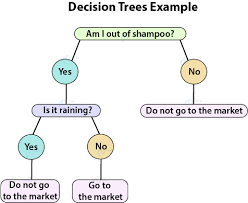
\includegraphics{DecTreeEg.png}
\caption{\ul{Decision Tree Example
(}\href{https://data-flair.training/blogs/r-decision-trees/}{Source})}
\end{figure}

\hypertarget{pre-processing-the-data}{%
\subsection{Pre-processing the data}\label{pre-processing-the-data}}

For this data, we will be dealing with the Status variable. The Status
variable was divided into 3 classes:

\begin{itemize}
\tightlist
\item
  Class 0 (D): The patient didn't survive by the end of the observation
\item
  Class 1 (C): The patient is censored, meaning that the observation
  period ended without the death being recorded
\item
  Class 2 (CL): Similar to Class 1, the patient is censored due to liver
  transplantation
\end{itemize}

Thus, we can group Class 1 and 2.

\begin{Shaded}
\begin{Highlighting}[]
\CommentTok{\#Combine C and CL status into one variable and binarize}
\NormalTok{cirrhosisTreeData }\OtherTok{\textless{}{-}}\NormalTok{ cirrhosis}
\NormalTok{cirrhosisTreeData}\SpecialCharTok{$}\NormalTok{Status }\OtherTok{\textless{}{-}} \FunctionTok{ifelse}\NormalTok{(cirrhosisTreeData}\SpecialCharTok{$}\NormalTok{Status }\SpecialCharTok{==} \StringTok{"C"} \SpecialCharTok{|}\NormalTok{ cirrhosisTreeData}\SpecialCharTok{$}\NormalTok{Status }\SpecialCharTok{==} \StringTok{"CL"}\NormalTok{, }\DecValTok{1}\NormalTok{, }\DecValTok{0}\NormalTok{)}
\end{Highlighting}
\end{Shaded}

\hypertarget{methodology}{%
\subsection{Methodology}\label{methodology}}

Our objective is to create a classifier capable of predicting a
patient's outcome. To achieve this, we will be testing our data with the
cart algorithm. To ensure model validation, we'll be using a 80\%
training and 20\% testing data division. I will also be stratifying the
data based on the status.

To guarantee consistency and reproducibility in our results, we have
fixed the seed for our 80/20 data split at 380. With these steps, we are
now well-positioned to finalize our training and testing data sets.

The predictors in these models will be guided by the results from the
EDA. We will also use a variety of tools to understand the model's
performance.

\begin{Shaded}
\begin{Highlighting}[]
\CommentTok{\# Wrangle the Graduate data to set up training and testing datasets}
\NormalTok{modelCirrhosis }\OtherTok{\textless{}{-}}\NormalTok{ cirrhosisTreeData }\SpecialCharTok{\%\textgreater{}\%}
  \CommentTok{\#drop\_na() \%\textgreater{}\%}
  \FunctionTok{mutate}\NormalTok{(}
    \AttributeTok{tempID =} \FunctionTok{row\_number}\NormalTok{(),}
    \AttributeTok{.before =}\NormalTok{ Status}
\NormalTok{  )}

\DocumentationTok{\#\# Set seed for reproducibility and slice {-}{-}{-}{-}}
\FunctionTok{set.seed}\NormalTok{(}\DecValTok{380}\NormalTok{)}
\NormalTok{trainingData }\OtherTok{\textless{}{-}}\NormalTok{ modelCirrhosis }\SpecialCharTok{\%\textgreater{}\%}
  \FunctionTok{group\_by}\NormalTok{(Status) }\SpecialCharTok{\%\textgreater{}\%}
  \FunctionTok{slice\_sample}\NormalTok{(}\AttributeTok{prop =} \FloatTok{0.8}\NormalTok{)}

\NormalTok{testingData }\OtherTok{\textless{}{-}}\NormalTok{ modelCirrhosis }\SpecialCharTok{\%\textgreater{}\%}
  \FunctionTok{filter}\NormalTok{(}\SpecialCharTok{!}\NormalTok{(tempID }\SpecialCharTok{\%in\%}\NormalTok{ trainingData}\SpecialCharTok{$}\NormalTok{tempID))}
\end{Highlighting}
\end{Shaded}

\hypertarget{step-1-growing-the-tree}{%
\subsubsection{Step 1: Growing the tree}\label{step-1-growing-the-tree}}

There are useful packages to build decision trees in R: the \{tree\} and
the \{rpart\} (recursive partitioning) packages.

In this report, I have decided to use \{rpart\} because it provides more
flexibility for surrogate splits and the trees are a bit easier to make
attractive looking.

\begin{Shaded}
\begin{Highlighting}[]
\CommentTok{\# Grow Graduate tree via rpart package}
\FunctionTok{library}\NormalTok{(rpart)}
\NormalTok{rPartStatus }\OtherTok{\textless{}{-}} \FunctionTok{rpart}\NormalTok{(}
  \AttributeTok{formula =}\NormalTok{ Status }\SpecialCharTok{\textasciitilde{}}\NormalTok{ Drug }\SpecialCharTok{+}\NormalTok{ Age }\SpecialCharTok{+}\NormalTok{ Sex }\SpecialCharTok{+}\NormalTok{ Ascites }\SpecialCharTok{+}\NormalTok{ Hepatomegaly }\SpecialCharTok{+}\NormalTok{ Spiders }\SpecialCharTok{+}\NormalTok{ Edema }\SpecialCharTok{+}\NormalTok{ Bilirubin }\SpecialCharTok{+}\NormalTok{ Cholesterol }\SpecialCharTok{+}\NormalTok{ Albumin }\SpecialCharTok{+}\NormalTok{ Copper }\SpecialCharTok{+}\NormalTok{ Alk\_Phos }\SpecialCharTok{+}\NormalTok{ SGOT }\SpecialCharTok{+}\NormalTok{ Platelets }\SpecialCharTok{+}\NormalTok{ Prothrombin }\SpecialCharTok{+}\NormalTok{ Stage }\SpecialCharTok{+}\NormalTok{ Tryglicerides, }
  \AttributeTok{data =}\NormalTok{ trainingData,}
  \AttributeTok{method =} \StringTok{"class"}\NormalTok{,}
  \AttributeTok{parms =} \FunctionTok{list}\NormalTok{(}\AttributeTok{split =} \StringTok{"information"}\NormalTok{)}
  \CommentTok{\# We did not need to use the control parameters}
\NormalTok{)}
\end{Highlighting}
\end{Shaded}

\hypertarget{part-2-visualizing-the-tree}{%
\subsubsection{Part 2: Visualizing the
tree}\label{part-2-visualizing-the-tree}}

With the tree grown, we can now visualize it for an easy understanding
of its functioning. This is an important advantage for CART over
logistic regression.

The following is a basic diagram for the tree that was just grown.

\begin{Shaded}
\begin{Highlighting}[]
\CommentTok{\# Display rpart.plot {-}{-}{-}{-}}
 \FunctionTok{library}\NormalTok{(rpart.plot)}
\FunctionTok{rpart.plot}\NormalTok{(}
  \AttributeTok{x =}\NormalTok{ rPartStatus,}
  \AttributeTok{type =} \DecValTok{2}\NormalTok{,}
  \AttributeTok{extra =} \DecValTok{101}
\NormalTok{)}
\end{Highlighting}
\end{Shaded}

\includegraphics{Submission_files/figure-latex/unnamed-chunk-22-1.pdf}

(Explanation of above) To gain a further understanding of the data, we
can plot a tree yielding Collection Node style trees. This can help us
understand how the data is split.

\begin{Shaded}
\begin{Highlighting}[]
\CommentTok{\# Using the rattle package to visualize the tree {-}{-}{-}{-}}
\FunctionTok{library}\NormalTok{(rattle)}
\end{Highlighting}
\end{Shaded}

\begin{verbatim}
## Loading required package: bitops
\end{verbatim}

\begin{verbatim}
## Rattle: A free graphical interface for data science with R.
## Version 5.5.1 Copyright (c) 2006-2021 Togaware Pty Ltd.
## Type 'rattle()' to shake, rattle, and roll your data.
\end{verbatim}

\begin{Shaded}
\begin{Highlighting}[]
\FunctionTok{fancyRpartPlot}\NormalTok{(}
  \AttributeTok{model =}\NormalTok{ rPartStatus,}
  \AttributeTok{main =} \ConstantTok{NULL}\NormalTok{,}
  \AttributeTok{sub =} \ConstantTok{NULL}
\NormalTok{)}
\end{Highlighting}
\end{Shaded}

\includegraphics{Submission_files/figure-latex/unnamed-chunk-23-1.pdf}

\hypertarget{part-3-pruning-the-tree}{%
\subsubsection{Part 3: Pruning the tree}\label{part-3-pruning-the-tree}}

Pruning reduces the size of decision trees by removing parts of the tree
that do not provide power to classify instances. The first step of
pruning a tree is understanding the complexity parameter used. The
complexity parameter (cp) in rpart is the minimum improvement in the
model needed at each node. This is used when building the tree. We can
see the results based on the cross validation from the table below.

\begin{Shaded}
\begin{Highlighting}[]
\FunctionTok{invisible}\NormalTok{(}\FunctionTok{capture.output}\NormalTok{(\{cpTable }\OtherTok{\textless{}{-}} \FunctionTok{printcp}\NormalTok{(rPartStatus)\}))}

\FunctionTok{library}\NormalTok{(kableExtra)}

\FunctionTok{kable}\NormalTok{(}
  \AttributeTok{x =}\NormalTok{ cpTable,}
  \AttributeTok{col.names =} \FunctionTok{c}\NormalTok{(}\StringTok{"CP"}\NormalTok{, }\StringTok{"Num. of splits"}\NormalTok{, }\StringTok{"Rel. Error"}\NormalTok{,}
                \StringTok{"Mean Error"}\NormalTok{, }\StringTok{"Std. Deviation of Error"}\NormalTok{),}
  \AttributeTok{digits =} \DecValTok{3}\NormalTok{,}
  \AttributeTok{booktabs =} \ConstantTok{TRUE}\NormalTok{,}
  \AttributeTok{align =} \StringTok{"c"}\NormalTok{,}
  \AttributeTok{table.attr =} \StringTok{\textquotesingle{}data{-}quarto{-}disable{-}processing="true"\textquotesingle{}}
\NormalTok{)}
\end{Highlighting}
\end{Shaded}

\begin{tabular}{ccccc}
\toprule
CP & Num. of splits & Rel. Error & Mean Error & Std. Deviation of Error\\
\midrule
0.375 & 0 & 1.000 & 1.000 & 0.069\\
0.109 & 1 & 0.625 & 0.711 & 0.064\\
0.035 & 2 & 0.516 & 0.695 & 0.063\\
0.023 & 4 & 0.445 & 0.633 & 0.061\\
0.020 & 5 & 0.422 & 0.641 & 0.061\\
\addlinespace
0.010 & 7 & 0.383 & 0.648 & 0.062\\
\bottomrule
\end{tabular}

This can also be visualized in a graph to gain a better understanding of
the data. The graph below shows the connection between the cp, size of
tree and the x-val relative error.

\begin{Shaded}
\begin{Highlighting}[]
\FunctionTok{plotcp}\NormalTok{(}
  \AttributeTok{x =}\NormalTok{ rPartStatus,}
  \AttributeTok{minline =} \ConstantTok{TRUE}\NormalTok{,}
  \AttributeTok{upper =} \StringTok{"size"}
\NormalTok{)}
\end{Highlighting}
\end{Shaded}

\includegraphics{Submission_files/figure-latex/unnamed-chunk-25-1.pdf}

From the graph we can see that a cp of 0.011 is ideal as it is under the
horizontal (dotted) reference line. We can prune the tree with this CP
value.

\begin{Shaded}
\begin{Highlighting}[]
\CommentTok{\# Prune the rpart Graduate Tree {-}{-}{-}{-}}
\NormalTok{rPartStatus2 }\OtherTok{\textless{}{-}} \FunctionTok{prune}\NormalTok{(}
  \AttributeTok{tree =}\NormalTok{ rPartStatus,}
  \AttributeTok{cp =} \FloatTok{0.029}
\NormalTok{)}
\end{Highlighting}
\end{Shaded}

We can plot the pruned tree

\begin{Shaded}
\begin{Highlighting}[]
\FunctionTok{fancyRpartPlot}\NormalTok{(}
  \AttributeTok{model =}\NormalTok{ rPartStatus2,}
  \AttributeTok{main =} \ConstantTok{NULL}\NormalTok{,}
  \AttributeTok{sub =} \ConstantTok{NULL}
\NormalTok{)}
\end{Highlighting}
\end{Shaded}

\includegraphics{Submission_files/figure-latex/unnamed-chunk-27-1.pdf}

\hypertarget{part-4-results}{%
\subsubsection{Part 4: Results}\label{part-4-results}}

Now, we can evaluate the results of the tree on the testing data from
the initial 80-20 split. As is true whenever we use validation
approaches, we need to test out our model on the testing data set. This
will give us a more accurate understanding of how well the model fits
the context we're seeking to build our understanding of.

An important part of our results is understanding the role of prediction
and inference. In a broad sense, prediction refers to the process of
making forecasts about future events or unknown values based on a model
while inference generally refers to the process of drawing conclusions
from data. For the basic tree, I will be mainly focusing on prediction
aspects of the results. However, later in the report, we will also be
exploring inference findings.

\begin{Shaded}
\begin{Highlighting}[]
\NormalTok{pred\_StatusRpart2 }\OtherTok{\textless{}{-}} \FunctionTok{predict}\NormalTok{(}
  \AttributeTok{object =}\NormalTok{ rPartStatus2,}
  \AttributeTok{newdata =}\NormalTok{ testingData,}
  \AttributeTok{type =} \StringTok{"prob"}
\NormalTok{)}

\CommentTok{\# Data Wrangling the predictions {-}{-}{-}{-}}
\NormalTok{StatusPrediction }\OtherTok{\textless{}{-}} \FunctionTok{data.frame}\NormalTok{(}
  \AttributeTok{rpart2\_non\_death =}\NormalTok{ pred\_StatusRpart2[, }\DecValTok{1}\NormalTok{],}
  \AttributeTok{rpart2\_death =}\NormalTok{ pred\_StatusRpart2[, }\DecValTok{2}\NormalTok{]}
\NormalTok{) }\SpecialCharTok{\%\textgreater{}\%}
  \FunctionTok{mutate}\NormalTok{(}
    \AttributeTok{rpart2\_pred =} \FunctionTok{ifelse}\NormalTok{(}
      \AttributeTok{test =}\NormalTok{ rpart2\_death }\SpecialCharTok{\textgreater{}}\NormalTok{ rpart2\_non\_death,}
      \AttributeTok{yes =} \DecValTok{1}\NormalTok{,}
      \AttributeTok{no =} \DecValTok{0}
\NormalTok{    )}
\NormalTok{  )}

\DocumentationTok{\#\# Set predictions as factors}
\NormalTok{StatusPrediction}\SpecialCharTok{$}\NormalTok{rpart2\_pred }\OtherTok{\textless{}{-}} \FunctionTok{as.factor}\NormalTok{(StatusPrediction}\SpecialCharTok{$}\NormalTok{rpart2\_pred)}

\CommentTok{\# Merge supervision column into predictions data frame {-}{-}{-}{-}}
\NormalTok{StatusPrediction }\OtherTok{\textless{}{-}} \FunctionTok{cbind}\NormalTok{(}
  \AttributeTok{tempID =}\NormalTok{ testingData}\SpecialCharTok{$}\NormalTok{tempID,}
  \AttributeTok{Status =}\NormalTok{ testingData}\SpecialCharTok{$}\NormalTok{Status,}
\NormalTok{  StatusPrediction}
\NormalTok{)}
\end{Highlighting}
\end{Shaded}

We can evaluate the results of this through a confusion matrix.

\begin{Shaded}
\begin{Highlighting}[]
\NormalTok{StatusPrediction}\SpecialCharTok{$}\NormalTok{Status }\OtherTok{\textless{}{-}} \FunctionTok{factor}\NormalTok{(StatusPrediction}\SpecialCharTok{$}\NormalTok{Status)}

\FunctionTok{library}\NormalTok{(yardstick)}
\end{Highlighting}
\end{Shaded}

\begin{verbatim}
## 
## Attaching package: 'yardstick'
\end{verbatim}

\begin{verbatim}
## The following object is masked from 'package:readr':
## 
##     spec
\end{verbatim}

\begin{Shaded}
\begin{Highlighting}[]
\CommentTok{\# Build confusion matrix for second tree model}
\NormalTok{conf\_matrix }\OtherTok{\textless{}{-}} \FunctionTok{conf\_mat}\NormalTok{(}
  \AttributeTok{data =}\NormalTok{ StatusPrediction,}
  \AttributeTok{truth =}\NormalTok{ Status,}
  \AttributeTok{estimate =}\NormalTok{ rpart2\_pred}
\NormalTok{)}\SpecialCharTok{$}\NormalTok{table}

\FunctionTok{kable}\NormalTok{(}
\NormalTok{  conf\_matrix,}
  \AttributeTok{col.names =} \FunctionTok{c}\NormalTok{(}\StringTok{"Prediction/Supervision"}\NormalTok{, }\StringTok{"0"}\NormalTok{, }\StringTok{"1"}\NormalTok{),}
  \AttributeTok{digits =} \DecValTok{3}\NormalTok{,}
  \AttributeTok{booktabs =} \ConstantTok{TRUE}\NormalTok{,}
  \AttributeTok{caption =} \StringTok{"Model 1: Confusion Matrix"}\NormalTok{,}
  \AttributeTok{align =} \StringTok{"c"}
\NormalTok{) }\SpecialCharTok{\%\textgreater{}\%}
\FunctionTok{kable\_styling}\NormalTok{(}\AttributeTok{latex\_options =} \StringTok{"HOLD\_position"}\NormalTok{)}
\end{Highlighting}
\end{Shaded}

\begin{table}[H]

\caption{\label{tab:unnamed-chunk-29}Model 1: Confusion Matrix}
\centering
\begin{tabular}[t]{lcc}
\toprule
Prediction/Supervision & 0 & 1\\
\midrule
0 & 19 & 9\\
1 & 14 & 43\\
\bottomrule
\end{tabular}
\end{table}

\begin{Shaded}
\begin{Highlighting}[]
\NormalTok{accuracy }\OtherTok{\textless{}{-}} \FunctionTok{accuracy}\NormalTok{(StatusPrediction, Status, rpart2\_pred)}
\NormalTok{specificity }\OtherTok{\textless{}{-}} \FunctionTok{specificity}\NormalTok{(StatusPrediction, Status, rpart2\_pred)}
\NormalTok{sensitivity }\OtherTok{\textless{}{-}} \FunctionTok{sensitivity}\NormalTok{(StatusPrediction, Status, rpart2\_pred)}
\end{Highlighting}
\end{Shaded}

\begin{Shaded}
\begin{Highlighting}[]
\CommentTok{\# Build a data frame with model metrics {-}{-}{-}{-}}
\NormalTok{StatusPreds }\OtherTok{\textless{}{-}}\NormalTok{ StatusPrediction }\SpecialCharTok{\%\textgreater{}\%}
\NormalTok{  dplyr}\SpecialCharTok{::}\FunctionTok{select}\NormalTok{(tempID, Status, }\FunctionTok{contains}\NormalTok{(}\StringTok{"\_pred"}\NormalTok{)) }\SpecialCharTok{\%\textgreater{}\%}
  \FunctionTok{pivot\_longer}\NormalTok{(}
    \AttributeTok{cols =} \SpecialCharTok{!}\FunctionTok{c}\NormalTok{(tempID, Status),}
    \AttributeTok{names\_to =} \StringTok{"model"}\NormalTok{,}
    \AttributeTok{values\_to =} \StringTok{"prediction"}
\NormalTok{  )}

\NormalTok{accuracy }\OtherTok{\textless{}{-}}\NormalTok{ StatusPreds }\SpecialCharTok{\%\textgreater{}\%}
  \FunctionTok{group\_by}\NormalTok{(model) }\SpecialCharTok{\%\textgreater{}\%}
  \FunctionTok{accuracy}\NormalTok{(}
    \AttributeTok{truth =}\NormalTok{ Status,}
    \AttributeTok{estimate =}\NormalTok{ prediction}
\NormalTok{  )}

\NormalTok{sensitivity }\OtherTok{\textless{}{-}}\NormalTok{ StatusPreds }\SpecialCharTok{\%\textgreater{}\%}
  \FunctionTok{group\_by}\NormalTok{(model) }\SpecialCharTok{\%\textgreater{}\%}
  \FunctionTok{sensitivity}\NormalTok{(}
    \AttributeTok{truth =}\NormalTok{ Status,}
    \AttributeTok{estimate =}\NormalTok{ prediction,}
    \AttributeTok{event\_level =} \StringTok{"second"}
\NormalTok{  )}

\NormalTok{specificity }\OtherTok{\textless{}{-}}\NormalTok{ StatusPreds }\SpecialCharTok{\%\textgreater{}\%}
  \FunctionTok{group\_by}\NormalTok{(model) }\SpecialCharTok{\%\textgreater{}\%}
  \FunctionTok{specificity}\NormalTok{(}
    \AttributeTok{truth =}\NormalTok{ Status,}
    \AttributeTok{estimate =}\NormalTok{ prediction,}
    \AttributeTok{event\_level =} \StringTok{"second"}
\NormalTok{  )}

\NormalTok{modelMetrics }\OtherTok{\textless{}{-}} \FunctionTok{bind\_rows}\NormalTok{(}
\NormalTok{  accuracy,}
\NormalTok{  sensitivity,}
\NormalTok{  specificity}
\NormalTok{)}
\end{Highlighting}
\end{Shaded}

From this, we can get the model's

\begin{itemize}
\item
  True Positive (TP): Predicted Graduated and actually Graduated. In
  this case, 2217
\item
  False Positive (FP): Predicted Graduated but actually Not Graduated.
  In this case, 1000
\item
  False Negative (FN): Predicted Not Graduated but actually Graduated.
  In this case, 244
\item
  True Negative (TN): Predicted Not Graduated and actually Not
  Graduated. In this case, 659
\end{itemize}

With this, we can also calculate the model's metrics.

\begin{Shaded}
\begin{Highlighting}[]
\CommentTok{\# Make a nice looking table of model metrics {-}{-}{-}{-}}
\NormalTok{modelMetrics }\SpecialCharTok{\%\textgreater{}\%}
\NormalTok{  dplyr}\SpecialCharTok{::}\FunctionTok{select}\NormalTok{(model, .metric, .estimate) }\SpecialCharTok{\%\textgreater{}\%}
  \FunctionTok{pivot\_wider}\NormalTok{(}
    \AttributeTok{id\_cols =}\NormalTok{ model,}
    \AttributeTok{names\_from =}\NormalTok{ .metric,}
    \AttributeTok{values\_from =}\NormalTok{ .estimate}
\NormalTok{  ) }\SpecialCharTok{\%\textgreater{}\%}
  \FunctionTok{kable}\NormalTok{(}
    \AttributeTok{digits =} \DecValTok{3}\NormalTok{,}
    \AttributeTok{booktabs =} \ConstantTok{TRUE}\NormalTok{,}
    \AttributeTok{align =} \StringTok{"c"}\NormalTok{,}
    \AttributeTok{table.attr =} \StringTok{\textquotesingle{}data{-}quarto{-}disable{-}processing="true"\textquotesingle{}}
\NormalTok{  )}
\end{Highlighting}
\end{Shaded}

\begin{tabular}{cccc}
\toprule
model & accuracy & sensitivity & specificity\\
\midrule
rpart2\_pred & 0.729 & 0.827 & 0.576\\
\bottomrule
\end{tabular}

\hypertarget{part-ii-exploring-the-predictors-for-the-patients-status-using-logistic-regression}{%
\section{Part II: Exploring the predictors for the patient's status
using logistic
regression}\label{part-ii-exploring-the-predictors-for-the-patients-status-using-logistic-regression}}

Next, let us explore our question with a different type of model and
compare the results with our tree. To do this, we will be using (binary)
logistic regression model.

\hypertarget{introduction-1}{%
\subsection{Introduction}\label{introduction-1}}

Logistic regression is a statistical method used for binary
classification, which predicts the probability of an outcome that can be
either true or false. This is done by understanding the relationship
between a dependent binary variable and one or more independent
variables. Logistic regression is easy to implement and interpret.
However there are also some drawbacks, the model assumes a linear
relationship between the independent variables and the log odds of the
dependent variable, which may not always hold true in complex real-world
scenarios. Furthermore, unlike the decision tree, linear regression
models cannot ignore N/A values.

\begin{figure}
\centering
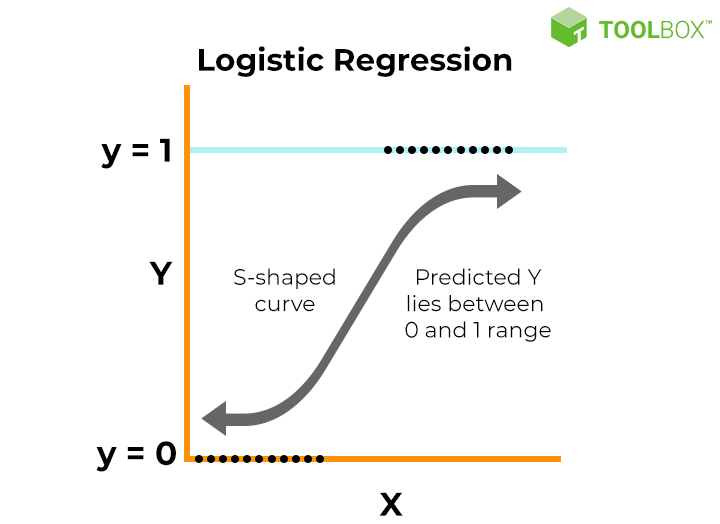
\includegraphics{46-4.png}
\caption{\ul{Logistic Regression Model
(\href{https://www.spiceworks.com/tech/artificial-intelligence/articles/what-is-logistic-regression/}{Source})}}
\end{figure}

\hypertarget{methodology-1}{%
\subsection{Methodology}\label{methodology-1}}

Similar to the tree, we will start by splitting the data set into
training and testing sets. Note that the data now only contains
instances where the patient was deceased. The training set will be used
to train our model, while the testing set will help evaluate its
performance. We'll use 80\% of the data for training and the remaining
20\% for testing. To allow reproducible code, we have fixed the seed at
380.

With this, we will build two candidate models:

\begin{itemize}
\item
  The first model will test the classification based on just the SGOT
\item
  The second model will use a step wise function using various
  predictors to see the best performance.
\end{itemize}

Another important consideration is the application of prediction
(estimating an outcome based on input variables) and inference
(understanding the relationships between variables). We will evaluate
the inference through the coefficient analysis and prediction through
roc curves and confusion matrix. It is important to note that these
metrics will complement each other in our understanding of the data.
However, the main focus of this analysis will be prediction and we will
work with several metrics to evaluate it.

We will use a variety of tools to understand the model's performance.

\begin{Shaded}
\begin{Highlighting}[]
\NormalTok{cirrhosisRegression }\OtherTok{\textless{}{-}}\NormalTok{ cirrhosis}
\NormalTok{cirrhosisRegression}\SpecialCharTok{$}\NormalTok{Status }\OtherTok{\textless{}{-}} \FunctionTok{ifelse}\NormalTok{(cirrhosisRegression}\SpecialCharTok{$}\NormalTok{Status }\SpecialCharTok{==} \StringTok{"C"} \SpecialCharTok{|}\NormalTok{ cirrhosisRegression}\SpecialCharTok{$}\NormalTok{Status }\SpecialCharTok{==} \StringTok{"CL"}\NormalTok{, }\DecValTok{1}\NormalTok{, }\DecValTok{0}\NormalTok{)}
\end{Highlighting}
\end{Shaded}

\begin{Shaded}
\begin{Highlighting}[]
\CommentTok{\#model data}
\NormalTok{LRmodelData }\OtherTok{\textless{}{-}}\NormalTok{ cirrhosisRegression }\SpecialCharTok{\%\textgreater{}\%}
  \FunctionTok{drop\_na}\NormalTok{() }\SpecialCharTok{\%\textgreater{}\%}
  \FunctionTok{mutate}\NormalTok{(}
    \AttributeTok{tempID =} \FunctionTok{row\_number}\NormalTok{(),}
    \AttributeTok{.before =}\NormalTok{ Status}
\NormalTok{  )}

\CommentTok{\# Set seed for reproducibility and slice}
\FunctionTok{set.seed}\NormalTok{(}\DecValTok{380}\NormalTok{)}
\NormalTok{trainingData }\OtherTok{\textless{}{-}}\NormalTok{ LRmodelData }\SpecialCharTok{\%\textgreater{}\%}
  \FunctionTok{group\_by}\NormalTok{(Status) }\SpecialCharTok{\%\textgreater{}\%}  \CommentTok{\# group\_by() function ensures that the data}
  \FunctionTok{slice\_sample}\NormalTok{(}\AttributeTok{prop =} \FloatTok{0.80}\NormalTok{)}

\NormalTok{testingData }\OtherTok{\textless{}{-}}\NormalTok{ LRmodelData }\SpecialCharTok{\%\textgreater{}\%}
  \FunctionTok{filter}\NormalTok{(}\SpecialCharTok{!}\NormalTok{(tempID }\SpecialCharTok{\%in\%}\NormalTok{ trainingData}\SpecialCharTok{$}\NormalTok{tempID))}

\NormalTok{trainingResults }\OtherTok{\textless{}{-}}\NormalTok{ trainingData}
\end{Highlighting}
\end{Shaded}

\begin{Shaded}
\begin{Highlighting}[]
\CommentTok{\# Form Candidate Model 1}
\NormalTok{model1 }\OtherTok{\textless{}{-}} \FunctionTok{glm}\NormalTok{(}
  \AttributeTok{formula =}\NormalTok{ Status }\SpecialCharTok{\textasciitilde{}}\NormalTok{ SGOT,}
  \AttributeTok{data =}\NormalTok{ trainingData,}
  \AttributeTok{family =}\NormalTok{ binomial}
\NormalTok{)}
\end{Highlighting}
\end{Shaded}

Stepwise results:

\begin{Shaded}
\begin{Highlighting}[]
\CommentTok{\# Lower bound (Intercept only)}
\NormalTok{lower }\OtherTok{\textless{}{-}} \FunctionTok{glm}\NormalTok{(}
  \AttributeTok{formula =}\NormalTok{ Status }\SpecialCharTok{\textasciitilde{}} \DecValTok{1}\NormalTok{,}
  \AttributeTok{data =}\NormalTok{ trainingData,}
  \AttributeTok{family =}\NormalTok{ binomial}
\NormalTok{)}

\CommentTok{\# Upper bound }
\NormalTok{upper }\OtherTok{\textless{}{-}} \FunctionTok{glm}\NormalTok{(}
  \AttributeTok{formula =}\NormalTok{ Status }\SpecialCharTok{\textasciitilde{}}\NormalTok{ Drug }\SpecialCharTok{+}\NormalTok{ Age }\SpecialCharTok{+}\NormalTok{ Sex }\SpecialCharTok{+}\NormalTok{ Ascites }\SpecialCharTok{+}\NormalTok{ Hepatomegaly }\SpecialCharTok{+}\NormalTok{ Spiders }\SpecialCharTok{+}\NormalTok{ Edema }\SpecialCharTok{+}\NormalTok{ Bilirubin }\SpecialCharTok{+}\NormalTok{ Cholesterol }\SpecialCharTok{+}\NormalTok{ Albumin }\SpecialCharTok{+}\NormalTok{ Copper }\SpecialCharTok{+}\NormalTok{ Alk\_Phos }\SpecialCharTok{+}\NormalTok{ SGOT }\SpecialCharTok{+}\NormalTok{ Platelets }\SpecialCharTok{+}\NormalTok{ Prothrombin }\SpecialCharTok{+}\NormalTok{ Stage,}
  \AttributeTok{data =}\NormalTok{ trainingData,}
  \AttributeTok{family =}\NormalTok{ binomial}
\NormalTok{)}


\CommentTok{\# Stepwise search}
\NormalTok{model2 }\OtherTok{\textless{}{-}} \FunctionTok{step}\NormalTok{(}
  \AttributeTok{object =}\NormalTok{ lower,}
  \AttributeTok{scope =} \FunctionTok{list}\NormalTok{(}
    \AttributeTok{lower =}\NormalTok{ lower,}
    \AttributeTok{upper =}\NormalTok{ upper}
\NormalTok{  ),}
  \AttributeTok{data =}\NormalTok{ trainingData,}
  \AttributeTok{direction =} \StringTok{"both"}\NormalTok{,}
  \AttributeTok{k =} \DecValTok{2}
\NormalTok{)}
\end{Highlighting}
\end{Shaded}

\begin{verbatim}
## Start:  AIC=298.13
## Status ~ 1
## 
##                Df Deviance    AIC
## + Bilirubin     1   247.26 251.26
## + Prothrombin   1   257.25 261.25
## + Copper        1   261.84 265.84
## + Edema         2   265.53 271.53
## + Ascites       1   273.57 277.57
## + Stage         3   270.16 278.16
## + Albumin       1   274.21 278.21
## + Alk_Phos      1   274.91 278.91
## + Hepatomegaly  1   275.05 279.05
## + Age           1   275.43 279.43
## + Spiders       1   278.02 282.02
## + SGOT          1   286.47 290.47
## + Platelets     1   291.25 295.25
## + Cholesterol   1   291.70 295.70
## + Sex           1   292.37 296.37
## + Drug          1   293.91 297.91
## <none>              296.12 298.12
## 
## Step:  AIC=251.26
## Status ~ Bilirubin
## 
##                Df Deviance    AIC
## + Age           1   225.30 231.30
## + Prothrombin   1   226.27 232.27
## + Alk_Phos      1   233.06 239.06
## + Edema         2   231.75 239.75
## + Albumin       1   238.01 244.01
## + Ascites       1   238.45 244.45
## + Stage         3   235.74 245.74
## + Copper        1   240.06 246.06
## + Spiders       1   241.63 247.63
## + Hepatomegaly  1   242.06 248.06
## + Platelets     1   243.87 249.87
## + Sex           1   244.21 250.21
## + Drug          1   244.37 250.37
## + Cholesterol   1   245.13 251.13
## <none>              247.26 251.26
## + SGOT          1   247.14 253.14
## - Bilirubin     1   296.12 298.12
## 
## Step:  AIC=231.3
## Status ~ Bilirubin + Age
## 
##                Df Deviance    AIC
## + Alk_Phos      1   209.76 217.76
## + Prothrombin   1   212.33 220.33
## + Edema         2   213.68 223.68
## + Copper        1   218.03 226.03
## + Spiders       1   218.93 226.93
## + Albumin       1   219.94 227.94
## + Ascites       1   220.76 228.76
## + Stage         3   217.58 229.58
## + Hepatomegaly  1   221.76 229.76
## + SGOT          1   222.78 230.78
## <none>              225.30 231.30
## + Platelets     1   223.57 231.57
## + Drug          1   223.83 231.83
## + Cholesterol   1   224.86 232.86
## + Sex           1   225.06 233.06
## - Age           1   247.26 251.26
## - Bilirubin     1   275.43 279.43
## 
## Step:  AIC=217.76
## Status ~ Bilirubin + Age + Alk_Phos
## 
##                Df Deviance    AIC
## + Prothrombin   1   197.16 207.16
## + Edema         2   198.44 210.44
## + Spiders       1   201.18 211.18
## + Stage         3   201.16 215.16
## + Ascites       1   205.18 215.18
## + Platelets     1   205.24 215.24
## + Copper        1   205.94 215.94
## + Hepatomegaly  1   206.62 216.62
## + Albumin       1   206.69 216.69
## <none>              209.76 217.76
## + SGOT          1   208.15 218.15
## + Cholesterol   1   208.82 218.82
## + Drug          1   208.84 218.84
## + Sex           1   209.68 219.68
## - Alk_Phos      1   225.30 231.30
## - Age           1   233.06 239.06
## - Bilirubin     1   251.55 257.55
## 
## Step:  AIC=207.16
## Status ~ Bilirubin + Age + Alk_Phos + Prothrombin
## 
##                Df Deviance    AIC
## + Spiders       1   191.39 203.39
## + Edema         2   189.41 203.41
## + Stage         3   188.90 204.90
## + Copper        1   193.94 205.94
## + Albumin       1   194.23 206.23
## + Hepatomegaly  1   194.37 206.37
## + SGOT          1   194.45 206.45
## + Drug          1   194.58 206.58
## + Platelets     1   194.95 206.95
## + Ascites       1   195.07 207.07
## <none>              197.16 207.16
## + Cholesterol   1   197.12 209.12
## + Sex           1   197.16 209.16
## - Prothrombin   1   209.76 217.76
## - Age           1   211.78 219.78
## - Alk_Phos      1   212.33 220.33
## - Bilirubin     1   225.31 233.31
## 
## Step:  AIC=203.39
## Status ~ Bilirubin + Age + Alk_Phos + Prothrombin + Spiders
## 
##                Df Deviance    AIC
## + Edema         2   185.35 201.35
## + SGOT          1   188.49 202.49
## + Drug          1   188.82 202.82
## + Copper        1   189.22 203.22
## + Albumin       1   189.33 203.33
## + Ascites       1   189.38 203.38
## <none>              191.39 203.39
## + Hepatomegaly  1   189.64 203.64
## + Stage         3   185.74 203.74
## + Platelets     1   189.96 203.96
## + Sex           1   191.13 205.13
## + Cholesterol   1   191.37 205.37
## - Spiders       1   197.16 207.16
## - Prothrombin   1   201.18 211.18
## - Age           1   207.34 217.34
## - Alk_Phos      1   208.03 218.03
## - Bilirubin     1   214.93 224.93
## 
## Step:  AIC=201.35
## Status ~ Bilirubin + Age + Alk_Phos + Prothrombin + Spiders + 
##     Edema
## 
##                Df Deviance    AIC
## + SGOT          1   181.77 199.77
## + Drug          1   182.57 200.57
## <none>              185.35 201.35
## + Copper        1   183.38 201.38
## + Albumin       1   183.48 201.48
## + Hepatomegaly  1   184.08 202.08
## + Stage         3   180.39 202.39
## + Platelets     1   184.40 202.40
## + Sex           1   185.10 203.10
## + Ascites       1   185.32 203.32
## + Cholesterol   1   185.35 203.35
## - Edema         2   191.39 203.39
## - Spiders       1   189.41 203.41
## - Prothrombin   1   192.56 206.56
## - Age           1   199.74 213.74
## - Alk_Phos      1   201.49 215.49
## - Bilirubin     1   206.71 220.71
## 
## Step:  AIC=199.77
## Status ~ Bilirubin + Age + Alk_Phos + Prothrombin + Spiders + 
##     Edema + SGOT
## 
##                Df Deviance    AIC
## + Drug          1   178.92 198.92
## <none>              181.77 199.77
## + Copper        1   179.90 199.90
## + Albumin       1   180.44 200.44
## + Hepatomegaly  1   180.66 200.66
## + Stage         3   177.01 201.01
## + Platelets     1   181.13 201.13
## - SGOT          1   185.35 201.35
## + Sex           1   181.53 201.53
## + Cholesterol   1   181.68 201.68
## + Ascites       1   181.70 201.70
## - Spiders       1   185.80 201.80
## - Edema         2   188.49 202.49
## - Prothrombin   1   189.92 205.92
## - Bilirubin     1   196.19 212.19
## - Alk_Phos      1   196.52 212.52
## - Age           1   198.70 214.70
## 
## Step:  AIC=198.92
## Status ~ Bilirubin + Age + Alk_Phos + Prothrombin + Spiders + 
##     Edema + SGOT + Drug
## 
##                Df Deviance    AIC
## + Copper        1   176.90 198.90
## <none>              178.92 198.92
## + Stage         3   173.10 199.10
## + Hepatomegaly  1   177.38 199.38
## + Albumin       1   177.49 199.49
## - Drug          1   181.77 199.77
## + Platelets     1   178.42 200.42
## - SGOT          1   182.57 200.57
## + Sex           1   178.69 200.69
## + Cholesterol   1   178.73 200.73
## - Spiders       1   182.83 200.83
## + Ascites       1   178.89 200.89
## - Edema         2   185.85 201.85
## - Prothrombin   1   188.64 206.64
## - Alk_Phos      1   193.00 211.00
## - Bilirubin     1   193.77 211.77
## - Age           1   194.21 212.21
## 
## Step:  AIC=198.9
## Status ~ Bilirubin + Age + Alk_Phos + Prothrombin + Spiders + 
##     Edema + SGOT + Drug + Copper
## 
##                Df Deviance    AIC
## <none>              176.90 198.90
## - Copper        1   178.92 198.92
## + Hepatomegaly  1   175.19 199.19
## + Albumin       1   175.31 199.31
## + Stage         3   171.76 199.76
## - Drug          1   179.90 199.90
## - Spiders       1   180.12 200.12
## + Platelets     1   176.38 200.38
## - SGOT          1   180.52 200.52
## + Ascites       1   176.82 200.82
## + Cholesterol   1   176.87 200.87
## + Sex           1   176.90 200.90
## - Edema         2   183.63 201.63
## - Bilirubin     1   184.57 204.57
## - Prothrombin   1   186.72 206.72
## - Alk_Phos      1   188.66 208.66
## - Age           1   191.54 211.54
\end{verbatim}

\hypertarget{results}{%
\section{Results}\label{results}}

Initially, we'll delve into the two preliminary models independently to
understand where they stand. Following that, we'll be deploying the best
candidate model on our test data. Regarding confusion matrices, we'll
employ a basic rule: if the predicted probability of a the patient's
status being ``deceased'' exceeds 0.5, we'll categorize them as deceased
(naïve rule).

\hypertarget{model-1}{%
\subsection{Model 1}\label{model-1}}

\begin{Shaded}
\begin{Highlighting}[]
\CommentTok{\# Model 1 Coefficient Table}
\FunctionTok{as.data.frame}\NormalTok{(}\FunctionTok{summary}\NormalTok{(model1)}\SpecialCharTok{$}\NormalTok{coefficients) }\SpecialCharTok{\%\textgreater{}\%}
  \FunctionTok{rownames\_to\_column}\NormalTok{(}\AttributeTok{var =} \StringTok{"X"}\NormalTok{) }\SpecialCharTok{\%\textgreater{}\%}
  \FunctionTok{rename}\NormalTok{(}\AttributeTok{coefficient =}\NormalTok{ Estimate) }\SpecialCharTok{\%\textgreater{}\%} 
  \FunctionTok{mutate}\NormalTok{(}
    \AttributeTok{prob\_odds =} \FunctionTok{case\_when}\NormalTok{(}
\NormalTok{      coefficient }\SpecialCharTok{==} \StringTok{"(Intercept)"} \SpecialCharTok{\textasciitilde{}} \FunctionTok{exp}\NormalTok{(coefficient)}\SpecialCharTok{/}\NormalTok{(}\DecValTok{1} \SpecialCharTok{+} \FunctionTok{exp}\NormalTok{(coefficient)),}
      \AttributeTok{.default =} \FunctionTok{exp}\NormalTok{(coefficient)}
\NormalTok{    ),}
    \AttributeTok{.after =}\NormalTok{ coefficient}
\NormalTok{  ) }\SpecialCharTok{\%\textgreater{}\%}
  \FunctionTok{mutate}\NormalTok{(}
    \StringTok{\textasciigrave{}}\AttributeTok{Pr(\textgreater{}|z|)}\StringTok{\textasciigrave{}} \OtherTok{=} \FunctionTok{ifelse}\NormalTok{(}
      \AttributeTok{test =} \StringTok{\textasciigrave{}}\AttributeTok{Pr(\textgreater{}|z|)}\StringTok{\textasciigrave{}} \SpecialCharTok{\textless{}} \FloatTok{0.001}\NormalTok{,}
      \AttributeTok{yes =} \FunctionTok{paste}\NormalTok{(}\StringTok{"\textless{} 0.001"}\NormalTok{),}
      \AttributeTok{no =} \StringTok{\textasciigrave{}}\AttributeTok{Pr(\textgreater{}|z|)}\StringTok{\textasciigrave{}}
\NormalTok{    ),}
    \AttributeTok{X =} \FunctionTok{case\_when}\NormalTok{(}
\NormalTok{      X }\SpecialCharTok{==} \StringTok{"(Intercept)"} \SpecialCharTok{\textasciitilde{}} \StringTok{"Intercept"}\NormalTok{,}
      \FunctionTok{grepl}\NormalTok{(}\AttributeTok{x =}\NormalTok{ X, }\AttributeTok{pattern =} \StringTok{"SGOT"}\NormalTok{) }\SpecialCharTok{\textasciitilde{}} \StringTok{"SGOT"}
\NormalTok{    )}
\NormalTok{  ) }\SpecialCharTok{\%\textgreater{}\%}
  \FunctionTok{kable}\NormalTok{()}
\end{Highlighting}
\end{Shaded}

\begin{tabular}{l|r|r|r|r|l}
\hline
X & coefficient & prob\_odds & Std. Error & z value & Pr(>|z|)\\
\hline
Intercept & 1.3728804 & 3.9467022 & 0.3566274 & 3.849622 & < 0.001\\
\hline
SGOT & -0.0077204 & 0.9923094 & 0.0026073 & -2.961056 & 0.00306586722502071\\
\hline
\end{tabular}

This table shows us the results of our first model. We can see that,
holding other variables constant, a one-unit increase in SGOT is
associated with a decrease in the log-odds of the response variable by
0.0076446. Furthermore, the odds-ratio indicates that for each one-unit
increase in SGOT, the odds of the event occurring decrease by about
0.76\%.

We can also plot the confusion matrix for this model:

\begin{Shaded}
\begin{Highlighting}[]
\FunctionTok{library}\NormalTok{(janitor)}
\end{Highlighting}
\end{Shaded}

\begin{verbatim}
## 
## Attaching package: 'janitor'
\end{verbatim}

\begin{verbatim}
## The following objects are masked from 'package:stats':
## 
##     chisq.test, fisher.test
\end{verbatim}

\begin{Shaded}
\begin{Highlighting}[]
\CommentTok{\# Building confidence intervals for Model 1 coefficients}
\NormalTok{model1CI }\OtherTok{\textless{}{-}} \FunctionTok{confint}\NormalTok{(}
  \AttributeTok{object =}\NormalTok{ model1,}
  \AttributeTok{parm =} \StringTok{"SGOT"}\NormalTok{,}
  \AttributeTok{level =} \FloatTok{0.9}
\NormalTok{)}
\end{Highlighting}
\end{Shaded}

\begin{verbatim}
## Waiting for profiling to be done...
\end{verbatim}

\begin{Shaded}
\begin{Highlighting}[]
\NormalTok{trainingResults }\OtherTok{\textless{}{-}}\NormalTok{ trainingData }\SpecialCharTok{\%\textgreater{}\%}
  \FunctionTok{ungroup}\NormalTok{() }\SpecialCharTok{\%\textgreater{}\%}
  \FunctionTok{mutate}\NormalTok{(}\AttributeTok{model1Pred =} \FunctionTok{predict}\NormalTok{(}\AttributeTok{object =}\NormalTok{ model1, }\AttributeTok{newdata =}\NormalTok{ ., }\AttributeTok{type =} \StringTok{"response"}\NormalTok{))}

\CommentTok{\# Apply naïve rule {-}{-}{-}{-}}
\NormalTok{trainingResults }\OtherTok{\textless{}{-}}\NormalTok{ trainingResults }\SpecialCharTok{\%\textgreater{}\%}
  \FunctionTok{mutate}\NormalTok{(}
    \AttributeTok{model1Class =} \FunctionTok{case\_when}\NormalTok{(}
\NormalTok{      model1Pred }\SpecialCharTok{\textgreater{}} \FloatTok{0.5} \SpecialCharTok{\textasciitilde{}} \StringTok{"Censored"}\NormalTok{,}
      \AttributeTok{.default =} \StringTok{"Deceased"}
\NormalTok{    )}
\NormalTok{  )}

\CommentTok{\#Confusion Matrix for Model 1}
\NormalTok{trainingResults }\SpecialCharTok{\%\textgreater{}\%}
  \FunctionTok{mutate}\NormalTok{(}\AttributeTok{Patient\_status =} \FunctionTok{ifelse}\NormalTok{(Status }\SpecialCharTok{==} \DecValTok{1}\NormalTok{, }\StringTok{"Censored"}\NormalTok{, }\StringTok{"Deceased"}\NormalTok{)) }\SpecialCharTok{\%\textgreater{}\%}
  \FunctionTok{tabyl}\NormalTok{(}\AttributeTok{var1 =}\NormalTok{ model1Class, }\AttributeTok{var2 =}\NormalTok{ Patient\_status) }\SpecialCharTok{\%\textgreater{}\%}
  \FunctionTok{adorn\_title}\NormalTok{(}
    \AttributeTok{placement =} \StringTok{"combined"}\NormalTok{,}
    \AttributeTok{row\_name =} \StringTok{"Predicted"}\NormalTok{,}
    \AttributeTok{col\_name =} \StringTok{"Actual"}
\NormalTok{  ) }\SpecialCharTok{\%\textgreater{}\%}
  \FunctionTok{kable}\NormalTok{(}
    \AttributeTok{booktabs =} \ConstantTok{TRUE}\NormalTok{,}
    \AttributeTok{align =} \StringTok{"c"}\NormalTok{,}
    \AttributeTok{caption =} \StringTok{"Model 1 Confusion Matrix"}
\NormalTok{  )}\SpecialCharTok{\%\textgreater{}\%}\FunctionTok{kable\_styling}\NormalTok{(}\AttributeTok{latex\_options =} \StringTok{"HOLD\_position"}\NormalTok{)}
\end{Highlighting}
\end{Shaded}

\begin{table}[H]

\caption{\label{tab:unnamed-chunk-36}Model 1 Confusion Matrix}
\centering
\begin{tabular}[t]{ccc}
\toprule
Predicted/Actual & Censored & Deceased\\
\midrule
Censored & 117 & 68\\
Deceased & 15 & 20\\
\bottomrule
\end{tabular}
\end{table}

We can see that this model tends to over predict censored values. This
shows the need of bringing in more factors. Next let us look at our
Model 2, which has multiple factors as discussed earlier.

\begin{Shaded}
\begin{Highlighting}[]
\CommentTok{\#Coeff for model 2}
\FunctionTok{as.data.frame}\NormalTok{(}\FunctionTok{summary}\NormalTok{(model2)}\SpecialCharTok{$}\NormalTok{coefficients) }\SpecialCharTok{\%\textgreater{}\%}
  \FunctionTok{rename}\NormalTok{(}\AttributeTok{coefficient =}\NormalTok{ Estimate) }\SpecialCharTok{\%\textgreater{}\%} 
  \FunctionTok{mutate}\NormalTok{(}
    \AttributeTok{prob\_odds =} \FunctionTok{case\_when}\NormalTok{(}
\NormalTok{      coefficient }\SpecialCharTok{==} \StringTok{"(Intercept)"} \SpecialCharTok{\textasciitilde{}} \FunctionTok{exp}\NormalTok{(coefficient)}\SpecialCharTok{/}\NormalTok{(}\DecValTok{1} \SpecialCharTok{+} \FunctionTok{exp}\NormalTok{(coefficient)),}
      \ConstantTok{TRUE} \SpecialCharTok{\textasciitilde{}} \FunctionTok{exp}\NormalTok{(coefficient)}
\NormalTok{    ),}
    \AttributeTok{.after =}\NormalTok{ coefficient}
\NormalTok{  ) }\SpecialCharTok{\%\textgreater{}\%}
  \FunctionTok{kable}\NormalTok{()}
\end{Highlighting}
\end{Shaded}

\begin{tabular}{l|r|r|r|r|r}
\hline
  & coefficient & prob\_odds & Std. Error & z value & Pr(>|z|)\\
\hline
(Intercept) & 13.1738171 & 5.264002e+05 & 2.5758130 & 5.1144306 & 0.0000003\\
\hline
Bilirubin & -0.2146715 & 8.068064e-01 & 0.0865790 & -2.4794883 & 0.0131571\\
\hline
Age & -0.0002039 & 9.997962e-01 & 0.0000571 & -3.5727423 & 0.0003533\\
\hline
Alk\_Phos & -0.0002988 & 9.997013e-01 & 0.0000968 & -3.0870015 & 0.0020219\\
\hline
Prothrombin & -0.6086022 & 5.441109e-01 & 0.2125486 & -2.8633552 & 0.0041918\\
\hline
Spiders & -0.7375877 & 4.782662e-01 & 0.4110588 & -1.7943606 & 0.0727556\\
\hline
EdemaS & -0.0940912 & 9.101997e-01 & 0.6115311 & -0.1538617 & 0.8777188\\
\hline
EdemaY & -16.3353205 & 1.000000e-07 & 857.1377366 & -0.0190580 & 0.9847948\\
\hline
SGOT & -0.0064630 & 9.935579e-01 & 0.0033599 & -1.9235635 & 0.0544093\\
\hline
DrugPlacebo & 0.6736154 & 1.961316e+00 & 0.3939801 & 1.7097702 & 0.0873084\\
\hline
Copper & -0.0038998 & 9.961078e-01 & 0.0027552 & -1.4154168 & 0.1569463\\
\hline
\end{tabular}

This analysis suggests significant associations between several
predictors (Bilirubin, Age, Alk\_Phos, Prothrombin, Spiders) and the
status of the patient. Each predictor, including the Intercept, shows a
statistically significant effect, as indicated by their small p-values
(Pr(\textgreater\textbar z\textbar)). The negative coefficients for
Bilirubin, Age, Alk\_Phos, Prothrombin, and Spiders imply that increases
in these variables are associated with a decrease in the log-odds of the
outcome. Bilirubin and Spiders are showing notably strong effects in the
model.

\begin{Shaded}
\begin{Highlighting}[]
\CommentTok{\#do the Tukey{-}Anscombe plot}
\FunctionTok{ggplot}\NormalTok{(}
  \AttributeTok{data =} \FunctionTok{data.frame}\NormalTok{(}
    \AttributeTok{residuals =} \FunctionTok{residuals}\NormalTok{(model2, }\AttributeTok{type =} \StringTok{"pearson"}\NormalTok{),}
    \AttributeTok{fitted =} \FunctionTok{fitted}\NormalTok{(model2)}
\NormalTok{  ),}
  \AttributeTok{mapping =} \FunctionTok{aes}\NormalTok{(}\AttributeTok{x =}\NormalTok{ fitted, }\AttributeTok{y =}\NormalTok{ residuals)}
\NormalTok{) }\SpecialCharTok{+}
  \FunctionTok{geom\_point}\NormalTok{() }\SpecialCharTok{+}
  \FunctionTok{geom\_smooth}\NormalTok{(}
    \AttributeTok{formula =}\NormalTok{ y }\SpecialCharTok{\textasciitilde{}}\NormalTok{ x,}
    \AttributeTok{method =}\NormalTok{ stats}\SpecialCharTok{::}\NormalTok{loess,}
    \AttributeTok{method.args =} \FunctionTok{list}\NormalTok{(}\AttributeTok{degree =} \DecValTok{1}\NormalTok{),}
    \AttributeTok{se =} \ConstantTok{FALSE}\NormalTok{,}
    \AttributeTok{linewidth =} \FloatTok{0.5}
\NormalTok{  ) }\SpecialCharTok{+}
  \FunctionTok{theme\_bw}\NormalTok{() }\SpecialCharTok{+}
  \FunctionTok{labs}\NormalTok{(}
    \AttributeTok{x =} \StringTok{"Fitted"}\NormalTok{,}
    \AttributeTok{y =} \StringTok{"Pearson Residuals"}
\NormalTok{  )}
\end{Highlighting}
\end{Shaded}

\includegraphics{Submission_files/figure-latex/unnamed-chunk-38-1.pdf}

This figure shows us the Tukey-Anscombe plot using Pearson residuals for
Model 2. In an ideal fit, the residuals should be evenly distributed
about zero with constant mean and variance. The shape of the line
suggests that the model is not capturing someunder lying structure in
the data, especially in extreme cases.

\begin{Shaded}
\begin{Highlighting}[]
\CommentTok{\#plot the gvif}
\FunctionTok{as.data.frame}\NormalTok{(car}\SpecialCharTok{::}\FunctionTok{vif}\NormalTok{(model2)) }\SpecialCharTok{\%\textgreater{}\%}
  \FunctionTok{kable}\NormalTok{(}
    \AttributeTok{digits =} \DecValTok{3}\NormalTok{,}
    \AttributeTok{align =} \StringTok{"lcccc"}\NormalTok{,}
    \AttributeTok{booktab =} \ConstantTok{TRUE}\NormalTok{,}
    \AttributeTok{format.args =} \FunctionTok{list}\NormalTok{(}\AttributeTok{big.mark =} \StringTok{","}\NormalTok{),}
    \AttributeTok{table.attr =} \StringTok{\textquotesingle{}data{-}quarto{-}disable{-}processing="true"\textquotesingle{}}\NormalTok{,}
    \AttributeTok{label =} \StringTok{"GVIF analsyis"}
\NormalTok{  )}
\end{Highlighting}
\end{Shaded}

\begin{tabular}{llcc}
\toprule
  & GVIF & Df & GVIF\textasciicircum{}(1/(2*Df))\\
\midrule
Bilirubin & 1.419 & 1 & 1.191\\
Age & 1.232 & 1 & 1.110\\
Alk\_Phos & 1.033 & 1 & 1.017\\
Prothrombin & 1.117 & 1 & 1.057\\
Spiders & 1.038 & 1 & 1.019\\
\addlinespace
Edema & 1.119 & 2 & 1.029\\
SGOT & 1.252 & 1 & 1.119\\
Drug & 1.091 & 1 & 1.044\\
Copper & 1.301 & 1 & 1.140\\
\bottomrule
\end{tabular}

The Variance Inflation Factor (VIF) values for the variables in the
model (Bilirubin, Age, Alk\_Phos, Prothrombin, Spiders) are all close to
1, indicating minimal multicollinearity. This means that these
predictors are relatively independent of each other, enhancing the
reliability of the model.

\begin{Shaded}
\begin{Highlighting}[]
\CommentTok{\#Store the predicted and actual values for Model 2}
\NormalTok{trainingResults}\SpecialCharTok{$}\NormalTok{model2Pred }\OtherTok{\textless{}{-}} \FunctionTok{predict}\NormalTok{(model2, }\AttributeTok{type =} \StringTok{"response"}\NormalTok{)}
\NormalTok{trainingResults}\SpecialCharTok{$}\NormalTok{model2Class }\OtherTok{\textless{}{-}} \FunctionTok{ifelse}\NormalTok{(trainingResults}\SpecialCharTok{$}\NormalTok{model2Pred }\SpecialCharTok{\textgreater{}} \FloatTok{0.5}\NormalTok{, }\StringTok{"Censored"}\NormalTok{, }\StringTok{"Deceased"}\NormalTok{)}
\NormalTok{trainingResults}\SpecialCharTok{$}\NormalTok{Actual }\OtherTok{\textless{}{-}} \FunctionTok{ifelse}\NormalTok{(trainingData}\SpecialCharTok{$}\NormalTok{Status }\SpecialCharTok{==} \DecValTok{1}\NormalTok{, }\StringTok{"Censored"}\NormalTok{, }\StringTok{"Deceased"}\NormalTok{)}

\CommentTok{\# Create confusion matrix using table}
\NormalTok{confusionMatrixRegression }\OtherTok{\textless{}{-}} \FunctionTok{table}\NormalTok{(}\AttributeTok{Predicted =}\NormalTok{ trainingResults}\SpecialCharTok{$}\NormalTok{model2Class, }\AttributeTok{Actual =}\NormalTok{ trainingResults}\SpecialCharTok{$}\NormalTok{Actual)}

\FunctionTok{kable}\NormalTok{(confusionMatrixRegression, }\AttributeTok{caption =} \StringTok{"Confusion matrix for Model 2"}\NormalTok{) }\SpecialCharTok{\%\textgreater{}\%}
  \FunctionTok{kable\_classic}\NormalTok{(}\AttributeTok{latex\_options =} \StringTok{"HOLD\_position"}\NormalTok{)}
\end{Highlighting}
\end{Shaded}

\begin{table}[H]

\caption{\label{tab:unnamed-chunk-40}Confusion matrix for Model 2}
\centering
\begin{tabular}[t]{l|r|r}
\hline
  & Censored & Deceased\\
\hline
Censored & 115 & 24\\
\hline
Deceased & 17 & 64\\
\hline
\end{tabular}
\end{table}

From this confusion matrix we can see the relationships between the True
Positive, True Negative, False Positive and False Negative values. From
this we can calculate:

\begin{itemize}
\item
  \textbf{Accuracy}: Approximately 81.36\%
\item
  \textbf{Recall}: Approximately 79.01\%
\item
  \textbf{Precision}: Approximately 72.73\%
\item
  \textbf{F1 Score}: Approximately 75.74\%
\end{itemize}

Lastly, let us look at the separation plots for each of the models.

\begin{Shaded}
\begin{Highlighting}[]
\FunctionTok{library}\NormalTok{(pROC)}
\end{Highlighting}
\end{Shaded}

\begin{verbatim}
## Type 'citation("pROC")' for a citation.
\end{verbatim}

\begin{verbatim}
## 
## Attaching package: 'pROC'
\end{verbatim}

\begin{verbatim}
## The following objects are masked from 'package:stats':
## 
##     cov, smooth, var
\end{verbatim}

\begin{Shaded}
\begin{Highlighting}[]
\FunctionTok{library}\NormalTok{(separationplot)}
\end{Highlighting}
\end{Shaded}

\begin{verbatim}
## Loading required package: RColorBrewer
\end{verbatim}

\begin{verbatim}
## Loading required package: Hmisc
\end{verbatim}

\begin{verbatim}
## 
## Attaching package: 'Hmisc'
\end{verbatim}

\begin{verbatim}
## The following objects are masked from 'package:dplyr':
## 
##     src, summarize
\end{verbatim}

\begin{verbatim}
## The following objects are masked from 'package:base':
## 
##     format.pval, units
\end{verbatim}

\begin{verbatim}
## Loading required package: MASS
\end{verbatim}

\begin{verbatim}
## 
## Attaching package: 'MASS'
\end{verbatim}

\begin{verbatim}
## The following object is masked from 'package:dplyr':
## 
##     select
\end{verbatim}

\begin{verbatim}
## Loading required package: foreign
\end{verbatim}

\begin{Shaded}
\begin{Highlighting}[]
\CommentTok{\# Fit ROC Curves for later}
\DocumentationTok{\#\# Model 1}
\NormalTok{model1ROC }\OtherTok{\textless{}{-}} \FunctionTok{roc}\NormalTok{(}
  \AttributeTok{formula =}\NormalTok{ Status }\SpecialCharTok{\textasciitilde{}}\NormalTok{ model1Pred,}
  \AttributeTok{data =}\NormalTok{ trainingResults}
\NormalTok{)}
\end{Highlighting}
\end{Shaded}

\begin{verbatim}
## Setting levels: control = 0, case = 1
\end{verbatim}

\begin{verbatim}
## Setting direction: controls < cases
\end{verbatim}

\begin{Shaded}
\begin{Highlighting}[]
\NormalTok{model1ROC\_df }\OtherTok{\textless{}{-}} \FunctionTok{data.frame}\NormalTok{(}
  \AttributeTok{threshold =}\NormalTok{ model1ROC}\SpecialCharTok{$}\NormalTok{thresholds,}
  \AttributeTok{sensitivity =}\NormalTok{ model1ROC}\SpecialCharTok{$}\NormalTok{sensitivities,}
  \AttributeTok{specificity =}\NormalTok{ model1ROC}\SpecialCharTok{$}\NormalTok{specificities,}
  \AttributeTok{model =} \StringTok{"Model 1"}
\NormalTok{)}
\DocumentationTok{\#\# Model 2}
\NormalTok{model2ROC }\OtherTok{\textless{}{-}} \FunctionTok{roc}\NormalTok{(}
  \AttributeTok{formula =}\NormalTok{ Status }\SpecialCharTok{\textasciitilde{}}\NormalTok{ model2Pred,}
  \AttributeTok{data =}\NormalTok{ trainingResults}
\NormalTok{)}
\end{Highlighting}
\end{Shaded}

\begin{verbatim}
## Setting levels: control = 0, case = 1
## Setting direction: controls < cases
\end{verbatim}

\begin{Shaded}
\begin{Highlighting}[]
\NormalTok{model2ROC\_df }\OtherTok{\textless{}{-}} \FunctionTok{data.frame}\NormalTok{(}
  \AttributeTok{threshold =}\NormalTok{ model2ROC}\SpecialCharTok{$}\NormalTok{thresholds,}
  \AttributeTok{sensitivity =}\NormalTok{ model2ROC}\SpecialCharTok{$}\NormalTok{sensitivities,}
  \AttributeTok{specificity =}\NormalTok{ model2ROC}\SpecialCharTok{$}\NormalTok{specificities,}
  \AttributeTok{model =} \StringTok{"Model 2"}
\NormalTok{)}
\end{Highlighting}
\end{Shaded}

\begin{Shaded}
\begin{Highlighting}[]
\CommentTok{\# Convert \textquotesingle{}Actual\textquotesingle{} column to numeric 0/1}
\NormalTok{trainingResults }\OtherTok{\textless{}{-}}\NormalTok{ trainingResults }\SpecialCharTok{\%\textgreater{}\%}
  \FunctionTok{mutate}\NormalTok{(}
    \AttributeTok{actualNum =} \FunctionTok{if\_else}\NormalTok{(Actual }\SpecialCharTok{==} \StringTok{"Deceased"}\NormalTok{, }\DecValTok{0}\NormalTok{, }\DecValTok{1}\NormalTok{)}
\NormalTok{  )}


\CommentTok{\#Sepeation Plot}
\FunctionTok{par}\NormalTok{(}\AttributeTok{mar =} \FunctionTok{c}\NormalTok{(}\DecValTok{4}\NormalTok{,}\DecValTok{0}\NormalTok{,}\DecValTok{0}\NormalTok{,}\DecValTok{0}\NormalTok{))}
\FunctionTok{separationplot}\NormalTok{(}
  \AttributeTok{pred =}\NormalTok{ trainingResults}\SpecialCharTok{$}\NormalTok{model1Pred, }
  \AttributeTok{actual =}\NormalTok{ trainingResults}\SpecialCharTok{$}\NormalTok{actualNum, }
  \AttributeTok{type =} \StringTok{"rect"}\NormalTok{,}
  \AttributeTok{line =} \ConstantTok{TRUE}\NormalTok{, }
  \AttributeTok{lwd2 =} \DecValTok{2}\NormalTok{,}
  \AttributeTok{show.expected =} \ConstantTok{TRUE}\NormalTok{, }
  \AttributeTok{newplot =} \ConstantTok{FALSE}\NormalTok{,}
  \AttributeTok{heading =} \StringTok{"Model 1"}
\NormalTok{)}
\end{Highlighting}
\end{Shaded}

\includegraphics{Submission_files/figure-latex/unnamed-chunk-42-1.pdf}

\begin{Shaded}
\begin{Highlighting}[]
\CommentTok{\#Sepeation Plot}
\FunctionTok{par}\NormalTok{(}\AttributeTok{mar =} \FunctionTok{c}\NormalTok{(}\DecValTok{4}\NormalTok{,}\DecValTok{0}\NormalTok{,}\DecValTok{0}\NormalTok{,}\DecValTok{0}\NormalTok{))}
\FunctionTok{separationplot}\NormalTok{(}
  \AttributeTok{pred =}\NormalTok{ trainingResults}\SpecialCharTok{$}\NormalTok{model2Pred, }
  \AttributeTok{actual =}\NormalTok{ trainingResults}\SpecialCharTok{$}\NormalTok{actualNum, }
  \AttributeTok{type =} \StringTok{"rect"}\NormalTok{,}
  \AttributeTok{line =} \ConstantTok{TRUE}\NormalTok{, }
  \AttributeTok{lwd2 =} \DecValTok{2}\NormalTok{,}
  \AttributeTok{show.expected =} \ConstantTok{TRUE}\NormalTok{, }
  \AttributeTok{newplot =} \ConstantTok{FALSE}\NormalTok{,}
  \AttributeTok{heading =} \StringTok{"Model 2"}
\NormalTok{)}
\end{Highlighting}
\end{Shaded}

\includegraphics{Submission_files/figure-latex/unnamed-chunk-43-1.pdf}

The separation plot assesses the the fit of the model by providing the
model's ability to predict occurrences with a high probability and
non-occurrences with low probability. The separation plot above
separation plot suggests that Model 2 has a reasonably good performance
in predicting the patient's status, especially for the observations on
the left-most side of the plot compared to Model 1 with the training
data. We will later compare this graph with the testing data.

Lastly, let us look at the ROC curves for bothe the models.

\begin{Shaded}
\begin{Highlighting}[]
\DocumentationTok{\#\# Merge into existing data frame}
\NormalTok{rocData }\OtherTok{\textless{}{-}} \FunctionTok{rbind}\NormalTok{(model1ROC\_df, model2ROC\_df)}

\DocumentationTok{\#\# AUC Data}
\NormalTok{aucData }\OtherTok{\textless{}{-}} \FunctionTok{data.frame}\NormalTok{(}
  \AttributeTok{model =} \FunctionTok{c}\NormalTok{(}\StringTok{"Model 1"}\NormalTok{, }\StringTok{"Model 2"}\NormalTok{),}
  \AttributeTok{auc =} \FunctionTok{c}\NormalTok{(model1ROC}\SpecialCharTok{$}\NormalTok{auc, model2ROC}\SpecialCharTok{$}\NormalTok{auc)}
\NormalTok{)}
\end{Highlighting}
\end{Shaded}

\begin{Shaded}
\begin{Highlighting}[]
\CommentTok{\#ROC plot}
\FunctionTok{ggplot}\NormalTok{(}
  \AttributeTok{data =}\NormalTok{ rocData,}
  \AttributeTok{mapping =} \FunctionTok{aes}\NormalTok{(}\AttributeTok{x =} \DecValTok{1} \SpecialCharTok{{-}}\NormalTok{ specificity, }\AttributeTok{y =}\NormalTok{ sensitivity, }\AttributeTok{color =}\NormalTok{ model)}
\NormalTok{) }\SpecialCharTok{+}
  \FunctionTok{geom\_path}\NormalTok{() }\SpecialCharTok{+}
  \FunctionTok{geom\_abline}\NormalTok{(}
    \AttributeTok{slope =} \DecValTok{1}\NormalTok{,}
    \AttributeTok{intercept =} \DecValTok{0}\NormalTok{,}
    \AttributeTok{linetype =} \StringTok{"dotted"}
\NormalTok{  ) }\SpecialCharTok{+}
  \FunctionTok{geom\_text}\NormalTok{(}
  \AttributeTok{inherit.aes =} \ConstantTok{FALSE}\NormalTok{,}
  \AttributeTok{data =}\NormalTok{ aucData,}
  \AttributeTok{mapping =} \FunctionTok{aes}\NormalTok{(}\AttributeTok{label =} \FunctionTok{paste}\NormalTok{(model, }\StringTok{"AUC: }\SpecialCharTok{\textbackslash{}n}\StringTok{"}\NormalTok{, }\FunctionTok{round}\NormalTok{(auc, }\DecValTok{3}\NormalTok{))),}
  \AttributeTok{x =} \FunctionTok{c}\NormalTok{(}\FloatTok{0.25}\NormalTok{, }\FloatTok{0.15}\NormalTok{),}
  \AttributeTok{y =} \FunctionTok{c}\NormalTok{(}\FloatTok{0.4}\NormalTok{, }\FloatTok{1.05}\NormalTok{)}
\NormalTok{)}
\end{Highlighting}
\end{Shaded}

\includegraphics{Submission_files/figure-latex/unnamed-chunk-45-1.pdf}

From the graphs we can interpret that:

Model 1: - Its ROC curve is above the line of no discrimination,
indicating that the model has some predictive capabilities. - The AUC is
0.64, which is better than random guessing but suggests there's room for
improvement.

Model 2: - The ROC curve for Model 2 is significantly above that of
Model 1, and much closer to the top-left corner, indicating better
predictive performance. - The AUC is 0.899, which suggests a good
classification performance, and it's notably better than Model 1. - Its
ability to discriminate between positive and negative classes is
superior to that of Model 1.

Lastly, let us plot our influence plot.

\begin{Shaded}
\begin{Highlighting}[]
\CommentTok{\# Influence Plot for Model 2}
\NormalTok{idCases }\OtherTok{\textless{}{-}}\NormalTok{ car}\SpecialCharTok{::}\FunctionTok{influencePlot}\NormalTok{(model2)}
\end{Highlighting}
\end{Shaded}

\includegraphics{Submission_files/figure-latex/unnamed-chunk-46-1.pdf}

The influence plot shows several data points with high leverage and
large residuals, indicating potential outliers. Some observations,
notably those labeled like ``149,'' have significant influence on the
regression model due to their Cook's D values.

\hypertarget{testing-our-model}{%
\section{Testing our model}\label{testing-our-model}}

Using our final model, we now turn to see how well this classifier does
on our testing data. Recall that we initally set the test data during
the train test split.

The confusion matrix below shows the performance of our model using the
naïve decision rule.

\begin{Shaded}
\begin{Highlighting}[]
\CommentTok{\# Set up testing data results}
\NormalTok{testingData }\OtherTok{\textless{}{-}}\NormalTok{ testingData }\SpecialCharTok{\%\textgreater{}\%}
  \FunctionTok{mutate}\NormalTok{(}
    \AttributeTok{gradNum =} \FunctionTok{case\_when}\NormalTok{(}
\NormalTok{      Status }\SpecialCharTok{==} \DecValTok{0} \SpecialCharTok{\textasciitilde{}} \DecValTok{0}\NormalTok{,}
\NormalTok{      Status }\SpecialCharTok{==} \DecValTok{1} \SpecialCharTok{\textasciitilde{}} \DecValTok{1}
\NormalTok{    ),}
    \AttributeTok{.after =}\NormalTok{ Status}
\NormalTok{  )}
\NormalTok{testingData}\SpecialCharTok{$}\NormalTok{predict }\OtherTok{\textless{}{-}} \FunctionTok{predict}\NormalTok{(}
  \AttributeTok{object =}\NormalTok{ model2,}
  \AttributeTok{newdata =}\NormalTok{ testingData,}
  \AttributeTok{type =} \StringTok{"response"}
\NormalTok{)}
\NormalTok{testingData }\OtherTok{\textless{}{-}}\NormalTok{ testingData }\SpecialCharTok{\%\textgreater{}\%}
  \FunctionTok{mutate}\NormalTok{(}
    \AttributeTok{model2Class =} \FunctionTok{case\_when}\NormalTok{(}
\NormalTok{      predict }\SpecialCharTok{\textgreater{}} \FloatTok{0.5} \SpecialCharTok{\textasciitilde{}} \StringTok{"Censored"}\NormalTok{,}
      \AttributeTok{.default =} \StringTok{"Deceased"}
\NormalTok{    )}
\NormalTok{  )}
\end{Highlighting}
\end{Shaded}

\begin{Shaded}
\begin{Highlighting}[]
\NormalTok{testingData}\SpecialCharTok{$}\NormalTok{Status }\OtherTok{\textless{}{-}} \FunctionTok{ifelse}\NormalTok{(testingData}\SpecialCharTok{$}\NormalTok{Status }\SpecialCharTok{==} \DecValTok{1}\NormalTok{, }\StringTok{"Censored"}\NormalTok{, }\StringTok{"Deceased"}\NormalTok{)}

\CommentTok{\# Build Confusion Matrix for Testing Data}
\NormalTok{testingData }\SpecialCharTok{\%\textgreater{}\%}
  \FunctionTok{tabyl}\NormalTok{(}\AttributeTok{var1 =}\NormalTok{ model2Class, }\AttributeTok{var2 =}\NormalTok{ Status) }\SpecialCharTok{\%\textgreater{}\%}
  \FunctionTok{adorn\_title}\NormalTok{(}
    \AttributeTok{placement =} \StringTok{"combined"}\NormalTok{,}
    \AttributeTok{row\_name =} \StringTok{"Predicted"}\NormalTok{,}
    \AttributeTok{col\_name =} \StringTok{"Actual"}
\NormalTok{  ) }\SpecialCharTok{\%\textgreater{}\%}
  \FunctionTok{kable}\NormalTok{(}
    \AttributeTok{caption =} \StringTok{"Confusion Matrix for Test data"}
\NormalTok{  )}
\end{Highlighting}
\end{Shaded}

\begin{table}

\caption{\label{tab:unnamed-chunk-48}Confusion Matrix for Test data}
\centering
\begin{tabular}[t]{l|r|r}
\hline
Predicted/Actual & Censored & Deceased\\
\hline
Censored & 30 & 13\\
\hline
Deceased & 3 & 10\\
\hline
\end{tabular}
\end{table}

\begin{itemize}
\item
  \textbf{Accuracy}: Approximately 71.43\%
\item
  \textbf{Recall}: Approximately 76.92\%
\item
  \textbf{Precision}: Approximately 43.48\%
\item
  \textbf{F1 Score}: Approximately 55.56\%
\end{itemize}

This shows that our model is has struggled with overfitting, with an
especially low precision score. We will discuss this in the comparison
with the tree model, but this is a limitation of our data size. Lastly,
we can plot the separation plot.

\begin{Shaded}
\begin{Highlighting}[]
\CommentTok{\#Sepeation Plot}
\FunctionTok{par}\NormalTok{(}\AttributeTok{mar =} \FunctionTok{c}\NormalTok{(}\DecValTok{4}\NormalTok{,}\DecValTok{0}\NormalTok{,}\DecValTok{0}\NormalTok{,}\DecValTok{0}\NormalTok{))}
\FunctionTok{separationplot}\NormalTok{(}
  \AttributeTok{pred =}\NormalTok{ testingData}\SpecialCharTok{$}\NormalTok{predict, }
  \AttributeTok{actual =}\NormalTok{ testingData}\SpecialCharTok{$}\NormalTok{gradNum, }
  \AttributeTok{type =} \StringTok{"rect"}\NormalTok{,}
  \AttributeTok{line =} \ConstantTok{TRUE}\NormalTok{, }
  \AttributeTok{lwd2 =} \DecValTok{2}\NormalTok{,}
  \AttributeTok{show.expected =} \ConstantTok{TRUE}\NormalTok{, }
  \AttributeTok{newplot =} \ConstantTok{FALSE}
\NormalTok{)}
\end{Highlighting}
\end{Shaded}

\includegraphics{Submission_files/figure-latex/unnamed-chunk-49-1.pdf}

\hypertarget{part-iii-exploring-the-sub-clusters-of-the-cirrhosis-data-using-unsupervised-learning}{%
\section{Part III: Exploring the sub-clusters of the cirrhosis data
using unsupervised
learning}\label{part-iii-exploring-the-sub-clusters-of-the-cirrhosis-data-using-unsupervised-learning}}

In this section, we sought to if there are sub-collections of patients.
We expect sub-collections to mimic medical definitions of the stages of
Biliary Cirrhosis but are curious to see if clustering can reveal some
newer observations.

\hypertarget{introduction-2}{%
\subsection{Introduction}\label{introduction-2}}

Biliary Cirrhosis patients are typically clustered in four main clusters
(\href{https://www.healthline.com/health/primary-biliary-cirrhosis\#stages}{Source}):

\begin{itemize}
\item
  Stage 1: There's inflammation and damage to the walls of medium-sized
  bile ducts.
\item
  Stage 2: There's blockage of the small bile ducts.
\item
  Stage 3: This stage marks the beginning of scarring.
\item
  Stage 4: Cirrhosis has developed. This permanent, severe, scarring and
  damage to the liver.
\end{itemize}

In this section we will be using clustering on our data. K-means
Clustering is an unsupervised learning technique where data points are
grouped based on their similarities. It's commonly used to identify
patterns and structures within datasets without prior knowledge of the
groups. The main advantage of clustering is its ability to discover
hidden patterns in data. However, a significant drawback is the
subjectivity in defining the `similarity' criteria, which can lead to
varying results and interpretations.

\href{https://medium.datadriveninvestor.com/k-means-clustering-4a700d4a4720}{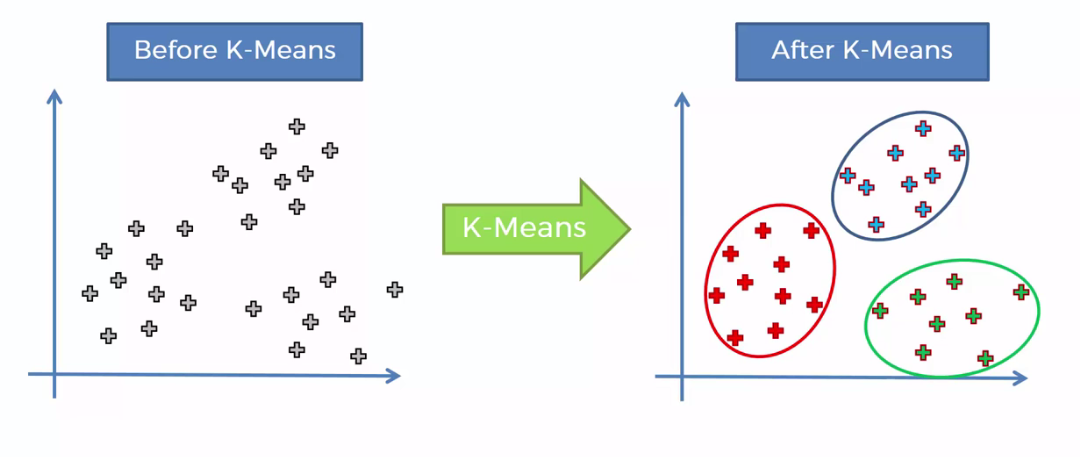
\includegraphics{1*fz-rjYPPRlGEMdTI-RLbDg.png}}

An important motivation for this part of the study is explore how does
``Stage'' which is typically defined based on medical professionals'
observations compares to the data that we have in this data set.

\hypertarget{pre-processing-the-data-1}{%
\subsection{Pre-processing the data}\label{pre-processing-the-data-1}}

We had to pre-process the data for the best performance. First, we
removed the `Stage' column to avoid using outcome-related features in
the unsupervised learning. The rows with N/A values were also removed.
Lastly, we transformed various categorical variables into numeric
formats, which is necessary for clustering algorithms.

\begin{Shaded}
\begin{Highlighting}[]
\CommentTok{\#do the ml, take about observational stages vs now quantify, look into the different variables and what they mean.}
\NormalTok{cirrhosisCluster }\OtherTok{\textless{}{-}}\NormalTok{ cirrhosis}

\NormalTok{cirrhosisCluster }\OtherTok{\textless{}{-}}\NormalTok{ cirrhosisCluster }\SpecialCharTok{\%\textgreater{}\%}                 
\NormalTok{                                  dplyr}\SpecialCharTok{::}\FunctionTok{select}\NormalTok{(}\SpecialCharTok{{-}}\NormalTok{Stage)     }
                                              
\NormalTok{cirrhosisCluster }\OtherTok{\textless{}{-}} \FunctionTok{na.omit}\NormalTok{(cirrhosisCluster) }\CommentTok{\#cannot have NA values in clustering}

\NormalTok{cirrhosisCluster}\SpecialCharTok{$}\NormalTok{Age\_Years }\OtherTok{\textless{}{-}} \FunctionTok{round}\NormalTok{(cirrhosisCluster}\SpecialCharTok{$}\NormalTok{Age\_Years) }\CommentTok{\#round age to whole numbers}


\CommentTok{\#reode sex... recode others later if need be \#female is 0}

\CommentTok{\#cirrhosisCluster  \textless{}{-} cirrhosisCluster \%\textgreater{}\%}
\CommentTok{\#  select( {-}c(Status, Drug, Edema)) \%\textgreater{}\%}
  
\CommentTok{\# mutate(Sex = ifelse(Sex == \textquotesingle{}Female\textquotesingle{}, 0, 1))}
     
      
\NormalTok{  cirrhosisCluster  }\OtherTok{\textless{}{-}}\NormalTok{ cirrhosisCluster }\SpecialCharTok{\%\textgreater{}\%}
    \FunctionTok{mutate}\NormalTok{(}\AttributeTok{Sex =} \FunctionTok{ifelse}\NormalTok{(Sex }\SpecialCharTok{==} \StringTok{\textquotesingle{}Female\textquotesingle{}}\NormalTok{, }\DecValTok{0}\NormalTok{, }\DecValTok{1}\NormalTok{)) }\SpecialCharTok{\%\textgreater{}\%}
          \FunctionTok{mutate}\NormalTok{(}\AttributeTok{Transplant =} \FunctionTok{ifelse}\NormalTok{(Status }\SpecialCharTok{==} \StringTok{"CL"}\NormalTok{, }\DecValTok{1}\NormalTok{, }\DecValTok{0}\NormalTok{)) }\SpecialCharTok{\%\textgreater{}\%}
              \FunctionTok{mutate}\NormalTok{(}\AttributeTok{Status =} \FunctionTok{ifelse}\NormalTok{(Status }\SpecialCharTok{\%in\%} \FunctionTok{c}\NormalTok{(}\StringTok{\textquotesingle{}C\textquotesingle{}}\NormalTok{, }\StringTok{\textquotesingle{}CL\textquotesingle{}}\NormalTok{), }\DecValTok{0}\NormalTok{ , }\DecValTok{1}\NormalTok{)) }\SpecialCharTok{\%\textgreater{}\%}
                    \FunctionTok{mutate}\NormalTok{(}\AttributeTok{Drug =} \FunctionTok{ifelse}\NormalTok{(Drug }\SpecialCharTok{==} \StringTok{"D{-}penicillamine"}\NormalTok{, }\DecValTok{0}\NormalTok{, }\DecValTok{1}\NormalTok{)) }\SpecialCharTok{\%\textgreater{}\%}
                        \FunctionTok{mutate}\NormalTok{(}\AttributeTok{EdemaDiurectics =} \FunctionTok{ifelse}\NormalTok{(Edema }\SpecialCharTok{\%in\%} \FunctionTok{c}\NormalTok{(}\StringTok{\textquotesingle{}S\textquotesingle{}}\NormalTok{, }\StringTok{\textquotesingle{}Y\textquotesingle{}}\NormalTok{), }\DecValTok{1}\NormalTok{, }\DecValTok{0}\NormalTok{)) }\SpecialCharTok{\%\textgreater{}\%}
                              \FunctionTok{mutate}\NormalTok{(}\AttributeTok{NoEdemaORD =} \FunctionTok{ifelse}\NormalTok{(Edema }\SpecialCharTok{==} \StringTok{\textquotesingle{}N\textquotesingle{}}\NormalTok{ , }\DecValTok{1}\NormalTok{, }\DecValTok{0}\NormalTok{)) }\SpecialCharTok{\%\textgreater{}\%}
                                        \FunctionTok{mutate}\NormalTok{(}\AttributeTok{EdemaANDD =} \FunctionTok{ifelse}\NormalTok{(Edema }\SpecialCharTok{==} \StringTok{"Y"}\NormalTok{, }\DecValTok{1}\NormalTok{, }\DecValTok{0}\NormalTok{)) }\SpecialCharTok{\%\textgreater{}\%}
                                                \FunctionTok{mutate}\NormalTok{(}\AttributeTok{EdemaORD =} \FunctionTok{ifelse}\NormalTok{(Edema }\SpecialCharTok{==} \StringTok{"S"}\NormalTok{, }\DecValTok{1}\NormalTok{, }\DecValTok{0}\NormalTok{)) }\SpecialCharTok{\%\textgreater{}\%}
\NormalTok{                                                                              dplyr}\SpecialCharTok{::}\FunctionTok{select}\NormalTok{(}\SpecialCharTok{{-}}\NormalTok{Edema)}
                                        
                                    
                          

\CommentTok{\#Data is already factored}
     
\CommentTok{\#mutate(Sex = ifelse(Sex == \textquotesingle{}Female\textquotesingle{}, 0, 1)) \%\textgreater{}\%}
  
   \CommentTok{\#mutate(Status = ifelse(Status \%in\% c(\textquotesingle{}C\textquotesingle{}, \textquotesingle{}CL\textquotesingle{}), 0 , 1)) \%\textgreater{}\%}
          \CommentTok{\#    mutate(Drug = ifelse(Drug == "D{-}penicillamine", 0, 1))}

  
\CommentTok{\#???:}
  
\CommentTok{\#make column yes no edema \#then yes no under treatment}

\CommentTok{\#same for transplant stuff}
\end{Highlighting}
\end{Shaded}

\begin{Shaded}
\begin{Highlighting}[]
\NormalTok{distCirrhosis }\OtherTok{\textless{}{-}} \FunctionTok{dist}\NormalTok{(}
  \AttributeTok{x =}\NormalTok{ cirrhosisCluster,}
  \AttributeTok{method =} \StringTok{"euclidean"}
\NormalTok{)}
\end{Highlighting}
\end{Shaded}

\hypertarget{methodology-2}{%
\subsection{Methodology}\label{methodology-2}}

To apply the k-means algorithm. A mixed hierarchical and
non-hierarchical was applied. This was done using the hkmeansm module,
with k = 4 as our initial value. Based on the data properties, the
euclidean (L2) distance works best.

\begin{Shaded}
\begin{Highlighting}[]
\NormalTok{hybridCirrhosis }\OtherTok{\textless{}{-}} \FunctionTok{hkmeans}\NormalTok{(}
  \AttributeTok{x =}\NormalTok{ cirrhosisCluster,}
  \AttributeTok{k =} \DecValTok{4}\NormalTok{,}
  \AttributeTok{hc.metric =} \StringTok{"euclidean"}\NormalTok{,}
  \AttributeTok{hc.method =} \StringTok{"ward.D"}\NormalTok{,}
  \AttributeTok{iter.max =} \DecValTok{10}
\NormalTok{)}
\end{Highlighting}
\end{Shaded}

\hypertarget{results-1}{%
\subsection{Results}\label{results-1}}

We were able to visualize the results of the k-means algorithm. The
first step was making a color palette and plotting the dendrogram tree.

\begin{Shaded}
\begin{Highlighting}[]
\NormalTok{StagesPalette }\OtherTok{\textless{}{-}} \FunctionTok{c}\NormalTok{(}\StringTok{"\#AA336A"}\NormalTok{, }\StringTok{"\#770737"}\NormalTok{, }\StringTok{"\#40B5AD"}\NormalTok{, }\StringTok{"\#009E60"}\NormalTok{, }\StringTok{"\#9FE2BF"}\NormalTok{)}
\end{Highlighting}
\end{Shaded}

\begin{Shaded}
\begin{Highlighting}[]
\DocumentationTok{\#\# MAKE A NEW PALLETE TO VISUALIZE}
\CommentTok{\# Plot the initial dendrogram for hybrid approach {-}{-}{-}{-}}
\FunctionTok{set.seed}\NormalTok{(}\DecValTok{380}\NormalTok{)}
\FunctionTok{hkmeans\_tree}\NormalTok{(}
  \AttributeTok{hkmeans =}\NormalTok{ hybridCirrhosis,}
  \AttributeTok{rect.col =}\NormalTok{ StagesPalette,}
  \AttributeTok{cex =} \FloatTok{0.4}\NormalTok{,}
  \AttributeTok{main =} \StringTok{"Initial Hierarchical Clusters"}
\NormalTok{)}
\end{Highlighting}
\end{Shaded}

\includegraphics{Submission_files/figure-latex/unnamed-chunk-54-1.pdf}

As, you can see, the model was able to create clear clusters for the
data. However, it is important to find the best value of k to get the
optimal clusters. To do this we can use a scree plot. Here,
we\textquotesingle re looking for the number of clusters that
corresponds to the "elbow".

\begin{Shaded}
\begin{Highlighting}[]
\CommentTok{\# Create scree plot for choosing k {-}{-}{-}{-}}
\FunctionTok{library}\NormalTok{(factoextra)}
\FunctionTok{set.seed}\NormalTok{(}\DecValTok{380}\NormalTok{)}
\FunctionTok{fviz\_nbclust}\NormalTok{(}
  \AttributeTok{x =}\NormalTok{ cirrhosisCluster,}
  \AttributeTok{diss =} \ConstantTok{NULL}\NormalTok{,}
  \AttributeTok{FUNcluster =}\NormalTok{ kmeans,}
  \AttributeTok{method =} \StringTok{"wss"}\NormalTok{,}
  \AttributeTok{k.max =} \DecValTok{10}
\NormalTok{)}
\end{Highlighting}
\end{Shaded}

\includegraphics{Submission_files/figure-latex/unnamed-chunk-55-1.pdf}

From this, we identified that 5 was the ideal value of k, where the
Total Within {[}Cluster{]} Sums of Squares begins leveling off. Let us
create a new k-means model with k = 5. We can plot this refined model,
with a format more easy to visualize.

\begin{Shaded}
\begin{Highlighting}[]
\NormalTok{hybridCirrhosis2 }\OtherTok{\textless{}{-}} \FunctionTok{hkmeans}\NormalTok{(}
  \AttributeTok{x =}\NormalTok{ cirrhosisCluster,}
  \AttributeTok{k =} \DecValTok{5}\NormalTok{,}
  \AttributeTok{hc.metric =} \StringTok{"euclidean"}\NormalTok{,}
  \AttributeTok{hc.method =} \StringTok{"ward.D"}\NormalTok{,}
  \AttributeTok{iter.max =} \DecValTok{10}
\NormalTok{)}
\end{Highlighting}
\end{Shaded}

\begin{Shaded}
\begin{Highlighting}[]
\CommentTok{\# Plot the final dendrogram for hybrid approach {-}{-}{-}{-}}
\CommentTok{\# library(factoextra)}
\FunctionTok{fviz\_dend}\NormalTok{(}
  \AttributeTok{x =}\NormalTok{ hybridCirrhosis2,}
  \AttributeTok{cex =} \FloatTok{0.4}\NormalTok{,}
  \AttributeTok{palette =}\NormalTok{ StagesPalette,}
  \AttributeTok{rect =} \ConstantTok{FALSE}\NormalTok{,}
  \AttributeTok{horiz =} \ConstantTok{TRUE}\NormalTok{,}
  \AttributeTok{repel =} \ConstantTok{TRUE}\NormalTok{,}
  \AttributeTok{main =} \StringTok{"Final Dendrogram"}
\NormalTok{)}
\end{Highlighting}
\end{Shaded}

\begin{verbatim}
## Warning: The `<scale>` argument of `guides()` cannot be `FALSE`. Use "none" instead as
## of ggplot2 3.3.4.
## i The deprecated feature was likely used in the factoextra package.
##   Please report the issue at <https://github.com/kassambara/factoextra/issues>.
## This warning is displayed once every 8 hours.
## Call `lifecycle::last_lifecycle_warnings()` to see where this warning was
## generated.
\end{verbatim}

\includegraphics{Submission_files/figure-latex/unnamed-chunk-57-1.pdf}

As you can see, the 5 clusters were identified, which are color coded in
our updated diagram.

Lastly, let us plot these clusters. Here is a plot of the initial model
where k = 4

\begin{Shaded}
\begin{Highlighting}[]
\CommentTok{\# Plot the final clustering for hybrid approach {-}{-}{-}{-}}
\CommentTok{\# library(factoextra)}
\FunctionTok{fviz\_cluster}\NormalTok{(}
  \AttributeTok{object =}\NormalTok{ hybridCirrhosis,}
  \AttributeTok{stand =} \ConstantTok{FALSE}\NormalTok{,}
  \AttributeTok{geom =} \StringTok{"point"}\NormalTok{,}
  \AttributeTok{main =} \StringTok{"Hybrid Cluster Plot {-} Initial model"}
\NormalTok{) }\SpecialCharTok{+}
  \FunctionTok{scale\_color\_manual}\NormalTok{(}\AttributeTok{values =}\NormalTok{ StagesPalette) }\SpecialCharTok{+}
  \FunctionTok{scale\_fill\_manual}\NormalTok{(}\AttributeTok{values =}\NormalTok{ StagesPalette) }\SpecialCharTok{+}
  \FunctionTok{theme\_bw}\NormalTok{() }
\end{Highlighting}
\end{Shaded}

\includegraphics{Submission_files/figure-latex/unnamed-chunk-58-1.pdf}

We can also plot our refined model, as you can see the plot below
identifies 5 clear clusters.

\begin{Shaded}
\begin{Highlighting}[]
\CommentTok{\# Plot the final clustering for hybrid approach {-}{-}{-}{-}}
\CommentTok{\# library(factoextra)}
\FunctionTok{fviz\_cluster}\NormalTok{(}
  \AttributeTok{object =}\NormalTok{ hybridCirrhosis2,}
  \AttributeTok{stand =} \ConstantTok{FALSE}\NormalTok{,}
  \AttributeTok{geom =} \StringTok{"point"}\NormalTok{,}
  \AttributeTok{main =} \StringTok{"Hybrid Cluster Plot {-} Refined model"}
\NormalTok{) }\SpecialCharTok{+}
  \FunctionTok{scale\_color\_manual}\NormalTok{(}\AttributeTok{values =}\NormalTok{ StagesPalette) }\SpecialCharTok{+}
  \FunctionTok{scale\_fill\_manual}\NormalTok{(}\AttributeTok{values =}\NormalTok{ StagesPalette) }\SpecialCharTok{+}
  \FunctionTok{theme\_bw}\NormalTok{() }
\end{Highlighting}
\end{Shaded}

\includegraphics{Submission_files/figure-latex/unnamed-chunk-59-1.pdf}

\end{document}
